\chapter{Simulations and Results}
	To test the performance of the guidance system, it is implemented in matlab/simulink. A number of
	scenarios are used to test how it performes in various conditions.

	The proposed system are greatly simplyfied and there are a number of situations that it will not work
	well. This situations are also threated and discussed in the next chapter. 
	

\section{Matlab}
	The mathematical model of the \textit{HUGIN 1000} AUV are implemented in simulink using the
	\textit{GNC} toolbox available from \textit{www.marinecontrol.org} with slight modifications to the
	6DOF model.

	The Camera output simulator were programmed in matlab. It inputs the position of the AUV and
	transposes it to body coordinates to calculate the field of view of the camera. The camera are based
	on the pinhole camera model with unity focus distance, and a view angle of about 45 degrees. The
	program then calculates the field of view of the camera and checks if there are any part of the
	pipeline inside the field of view. The output of the camera are three points taken out at the top, the
	middle and the bottom of the field of view.

	A sonar which determines the altitude are implemented using a look-up table with a predefined bottom
	profile.

	The descision logic is implemented as a state machine with three states, and gives out the 
	desired heading dependent on what state the system is in.

	The filter was created using a m-file and global variables for the filter parameters. The filter
	parameters are as follows:
	\begin{equation}
		P_0 = \left [ \begin{matrix}
				10 & 0 & 0 & 0 \\
				0 & 10 & 0 & 0 \\
				0 & 0 & 0.1 & 0 \\
				0 & 0 & 0 & 0.1
				\end{matrix} \right] \quad
		W = 0.1 \mathbf{I}_{2x2} \quad Q = 10 \mathbf{I}_{2x2} 
	\end{equation}

	The final simulink diagram are shown in figure \ref{fig:ch3_simulink}.
	\begin{figure}[htbp]
		\centering
		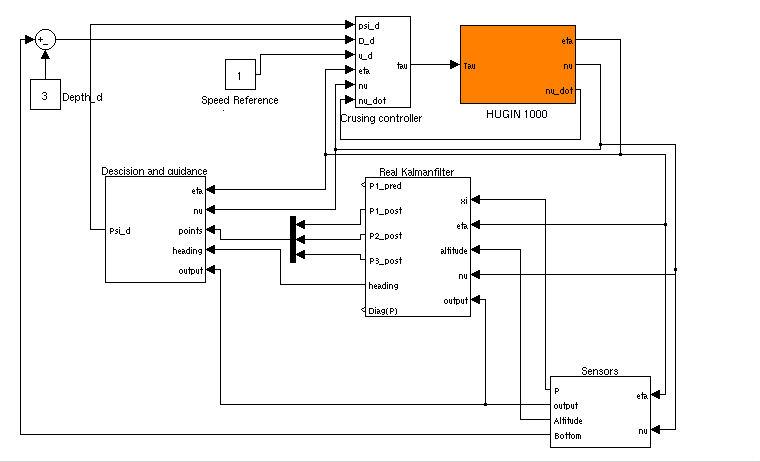
\includegraphics[width=\textwidth]{pics/simulink}
		\caption{The Simulink Diagram of the implemented Guidance System}
		\label{fig:ch3_simulink}
	\end{figure}

	

\section{Simulation Scenarios}
	To test the performance of the guidance system some scenarios are proposed. In all the scenarios the
	pipeline are located at the sea bottom around 10 meters bellow the surface. The AUV will start at the
	surface and submerge towards the starting point of the pipeline or the mission. 
	\begin{description}
		\item[\textbf{1$^{\mathrm{st}}$ Scenario}.] The pipeline are at the exact location acording 
		to predefined data. Environmental disturbances such as currents are turned off. The pipelien are
		continiously visible for the camera the whole inspection distance. Reference simulation.
		\item[\textbf{2$^{\mathrm{nd}}$ Scenario}.] Exact as over but with environmental forces turned on.
		\item[\textbf{3$^{\mathrm{rd}}$ Scenario}.] The pipeline are at the exact location where 
		it initially was layed. A section is burried, and not visible for the camera. Environmental
		forces are turned on.
		\item[\textbf{4$^{\mathrm{th}}$ Scenario}.] The \'a priori information about the pipeline 
		are offset about 20 meteres to test the ability of the guidance system to search for the pipeline.
	\end{description}


\section{Results}
	Some of the results for the simulations scenarios are given here. But first a test of the low-speed
	assumptions made for the controller design for the AUV. 

	\subsection{Test of the low-speed assumtion}
		In figures \ref{fig:ch3_coriolis_forces} and \ref{fig:ch3_damping_forces} the forces and
		moments created by the Coriolis/centripetal and damping matrices are recorded. In Figure
		\ref{fig:ch3_coriolis_forces} the sway degree of freedom are dominant, and peaking about
		-400N during the turning maneuvers of the AUV. The forces and moments created by the coriolis
		terms are partially counteracted by the damping terms, that also have greated magnitude than
		the coriolis terms.
		\begin{figure}[htbp]
			\centering
			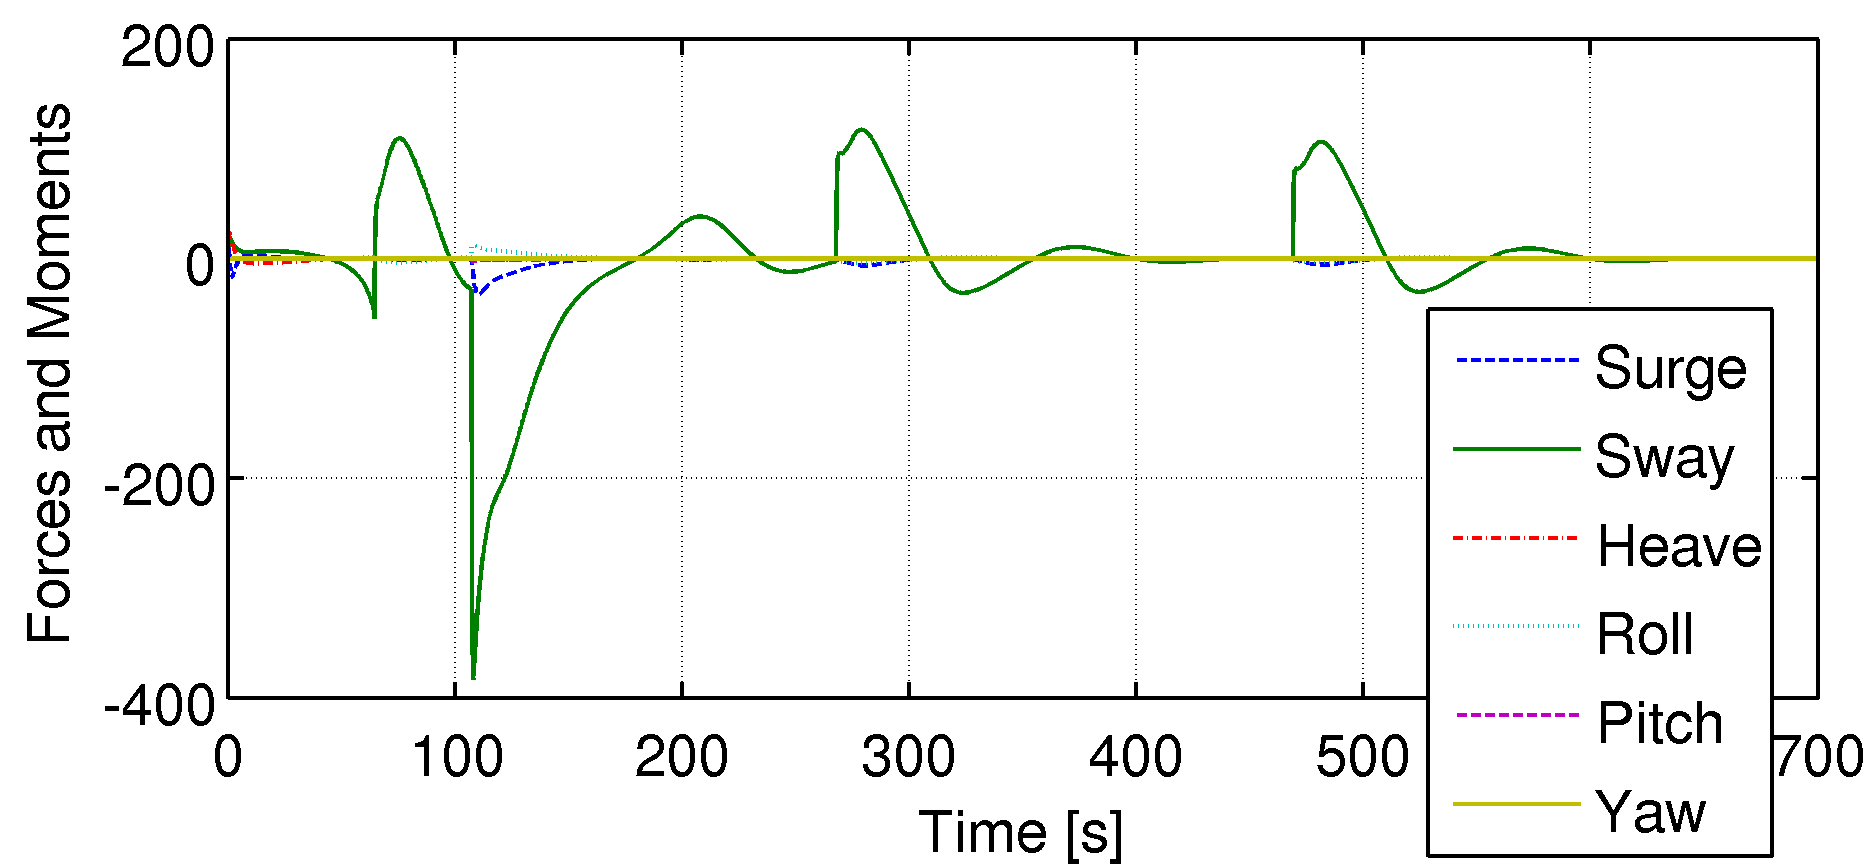
\includegraphics[width=0.7\textwidth]{pics/coriolis_forces}
			\caption{Plot of the Coriolis Forces Associated with the AUV Model}
			\label{fig:ch3_coriolis_forces}
		\end{figure}		
		\begin{figure}[htbp]
			\centering
			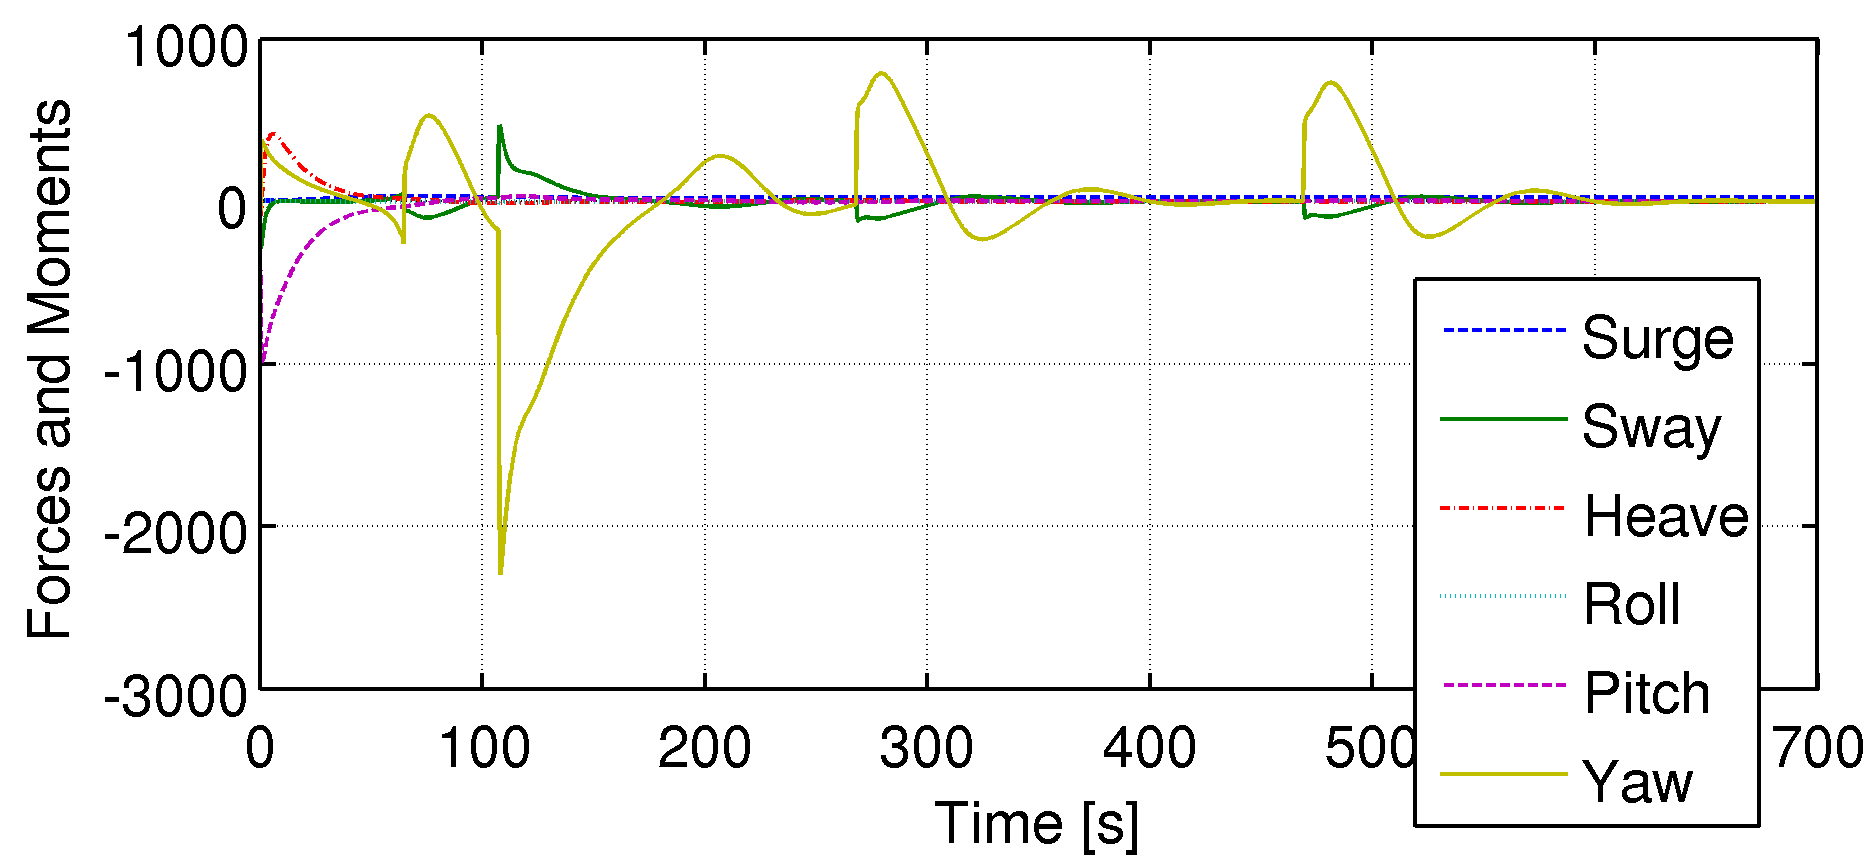
\includegraphics[width=0.7\textwidth]{pics/damping_forces}
			\caption{The Dampering Forces Associated with the AUV when Maneuvering}
			\label{fig:ch3_damping_forces}
		\end{figure}
		This suggests that the coriolis/centripetal forces can be neglected and compensated for as
		model errors in the controller using integral terms.  

	\subsection{1$^{\mathrm{st}}$ Scenario}
		This is mostly a reference test to see how the guidance system performs on the ideal case.
		This can show how sensitive the guidance system are with regard to current disturbances.
		\begin{figure}[htbp]
			\centering
			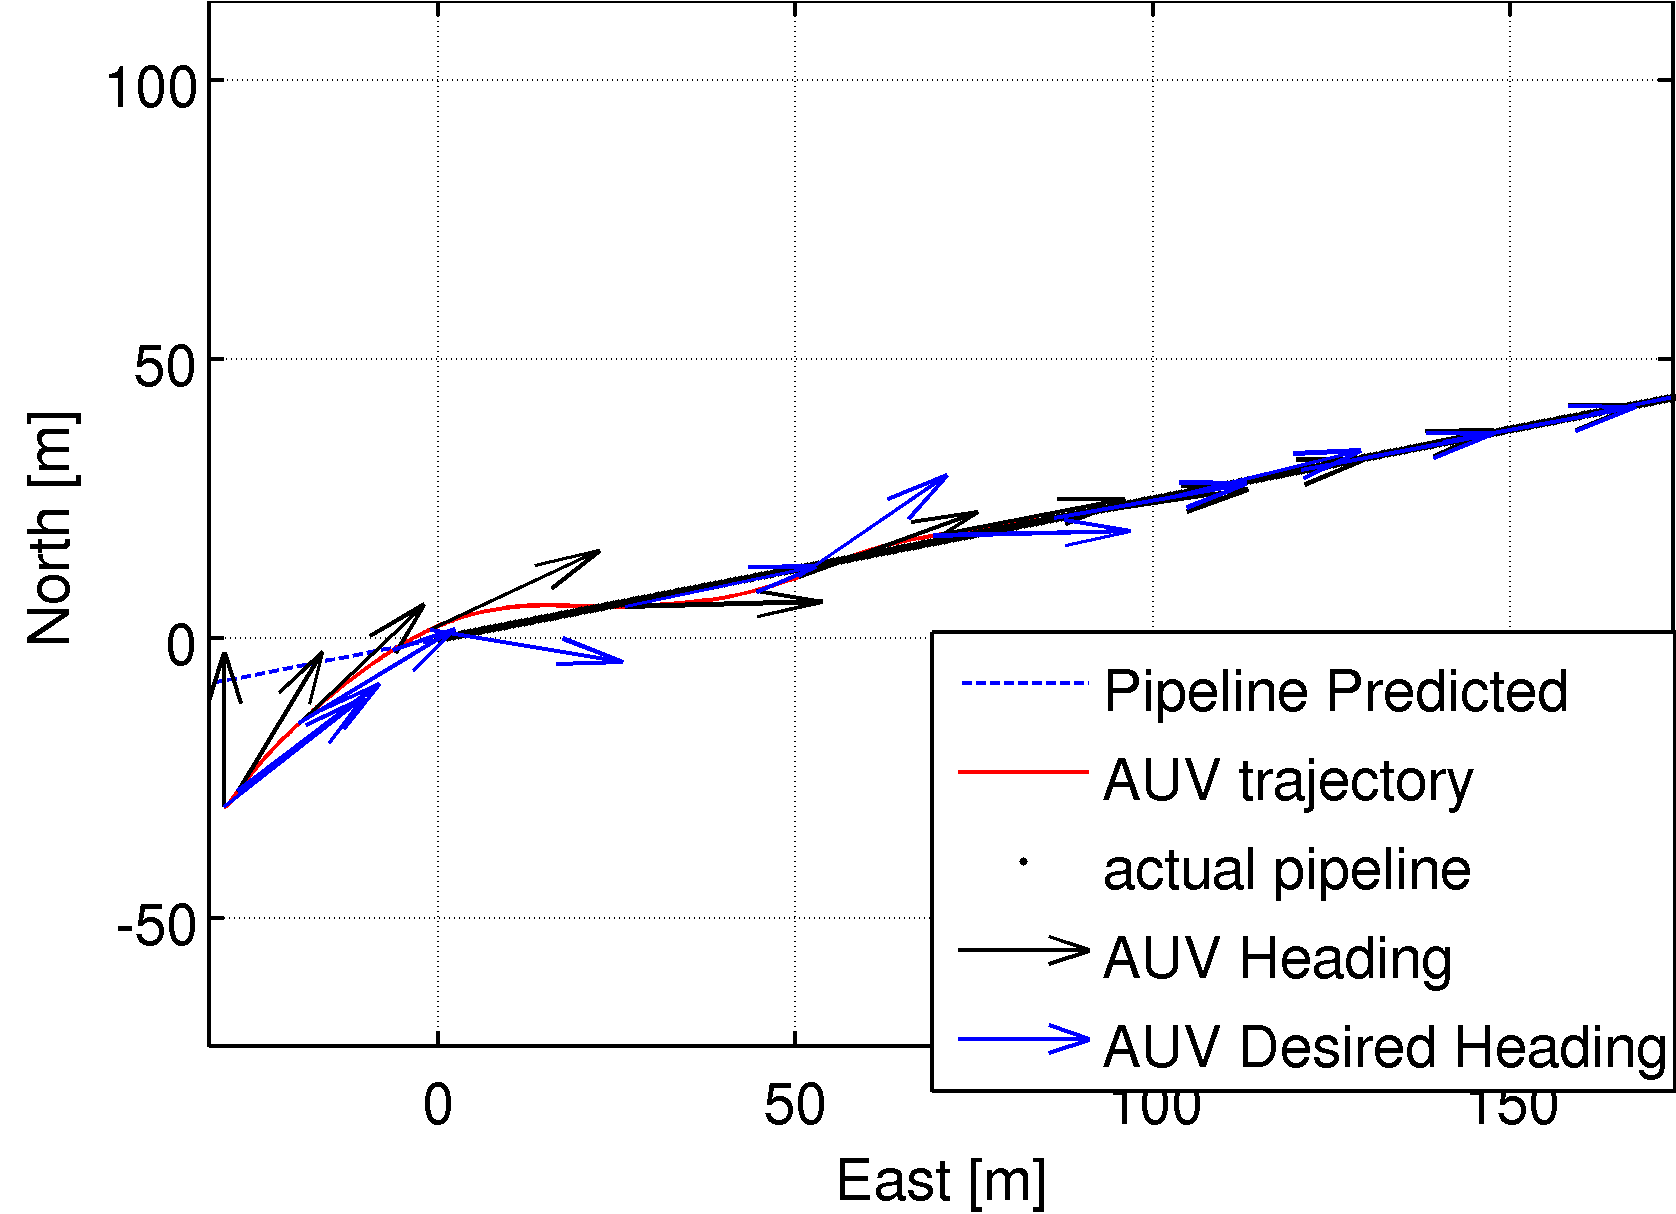
\includegraphics[width=0.7\textwidth]{pics/1st_NE_path}
			\caption{North East path of AUV without Current}
			\label{fig:ch3_1st_NE_path}
		\end{figure}
		\begin{figure}[htbp]
			\centering
			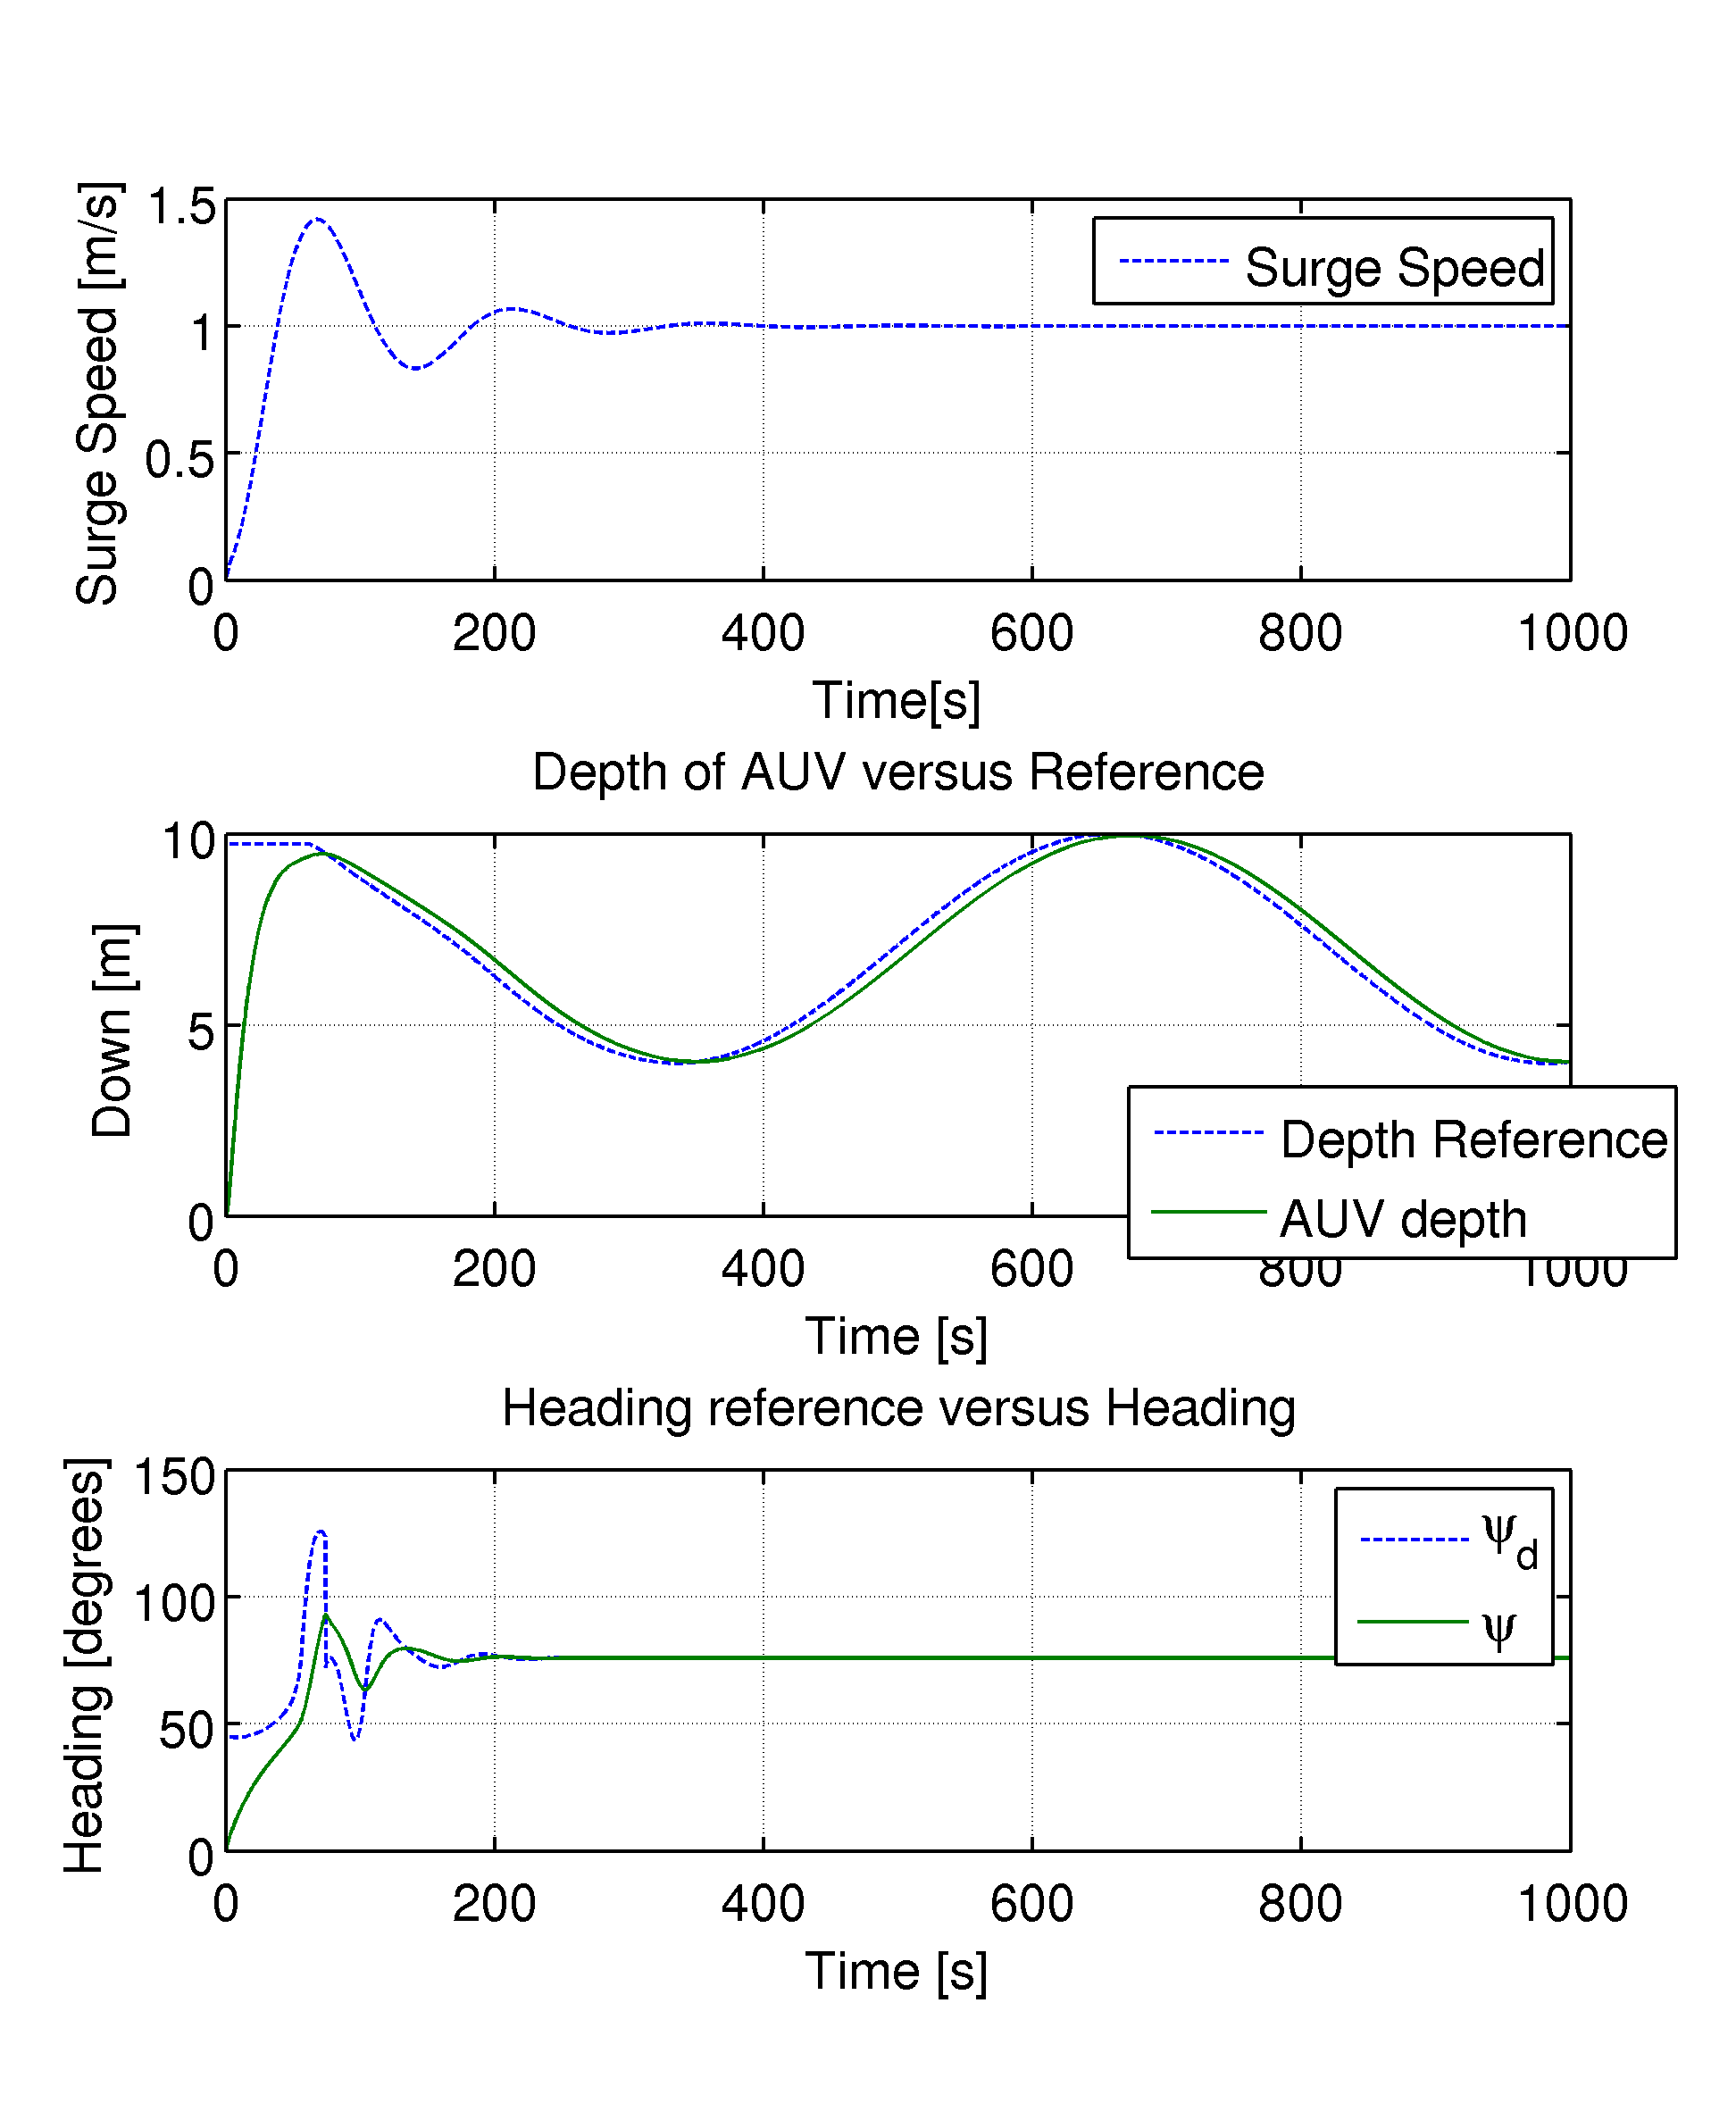
\includegraphics[width=0.75\textwidth]{pics/1st_uDpsi}
			\caption{Surge-, Depth- and Heading- Reference vs. Actual Values}
			\label{fig:ch3_1st_uDpsi}
		\end{figure}
		The result of this test is purly for reference but it might be an idea to notice some things
		about the simulations. 
		
		It can be seen from both Fiugre \ref{fig:ch3_1st_NE_path} and the
		third plot on Figure \ref{fig:ch3_1st_uDpsi} that the heading reference, $\psi_d$ have some
		oscilatory nature. This is because of the relatively low look-ahead distance defined in the
		guidance algorithm. This can be analogus to when driving a car and you fix your gaze on
		the road not very far ahead of the car, and you will get more uneasy driving and not so smooth motion. 

		The depth reference are given by the bottom which are constructed using a look-up table
		created by a sinuosidal plane. The reference are followed pretty well. The delay on the
		action by the controller are created because the \textit{heave} direction are not directley
		controlled, but are relayed through the \textit{pitch} degree of freedom. This could probably
		have been reduced by feeding the reference into the controller as well. This will help the
		controller predict the motion and compensate for it when it happens.

	
	\subsection{2$^{\mathrm{nd}}$ Scenario}
		The environmental forces are now turned. The current is assumed only effective in the North
		East plane and has no effect in the \textit{heave}-direction. The current is moving from
		north-west to south-east, heading $-45^{\circ}$ and have a strength of $0.3$ m/s. 
		
		\begin{figure}[htbp]
			\subfigure[NE Path with	Waypoints]{\label{fig:ch3_2nd_NE_wpt}
				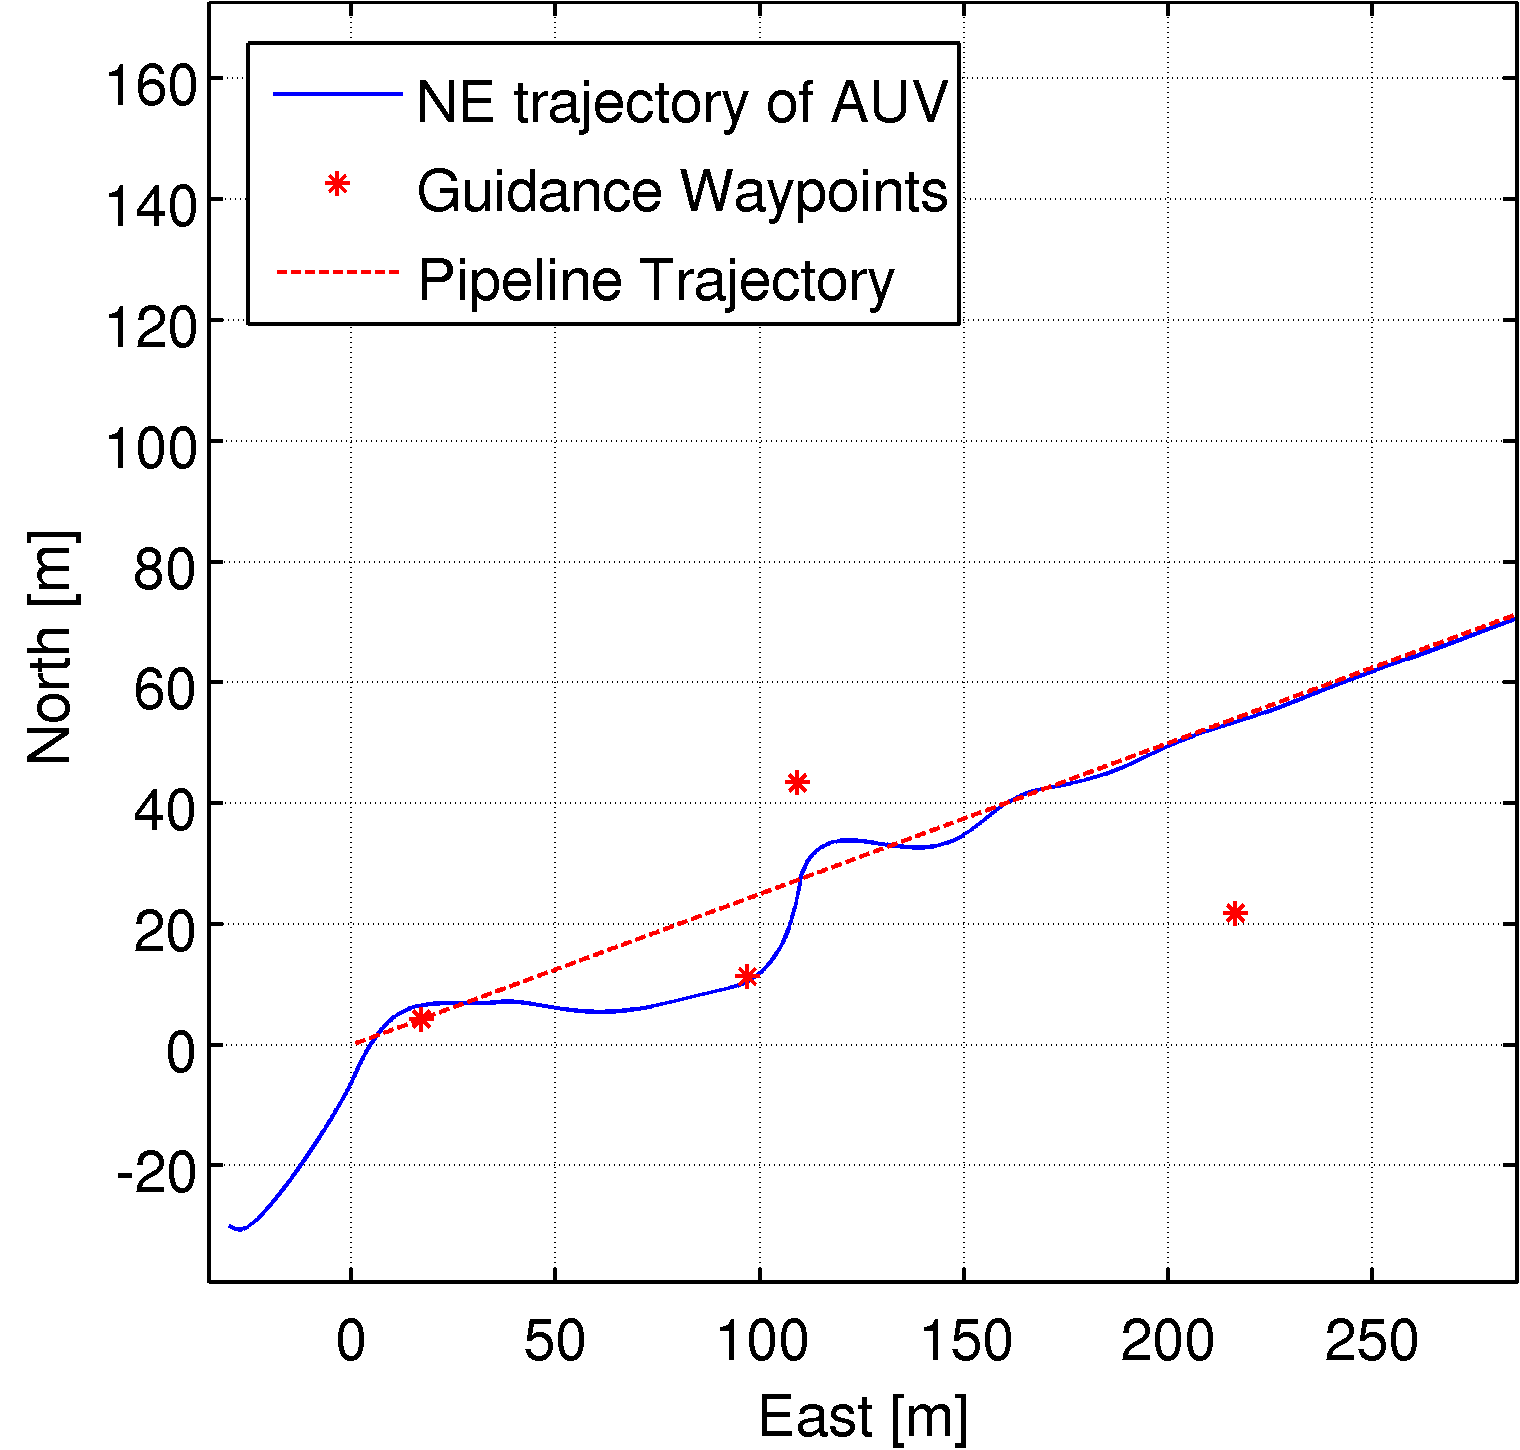
\includegraphics[width=0.5\textwidth]{pics/2nd_NE_wpt}}
			\subfigure[NE path with	Heading]{\label{fig:ch3_2nd_NE_path}
				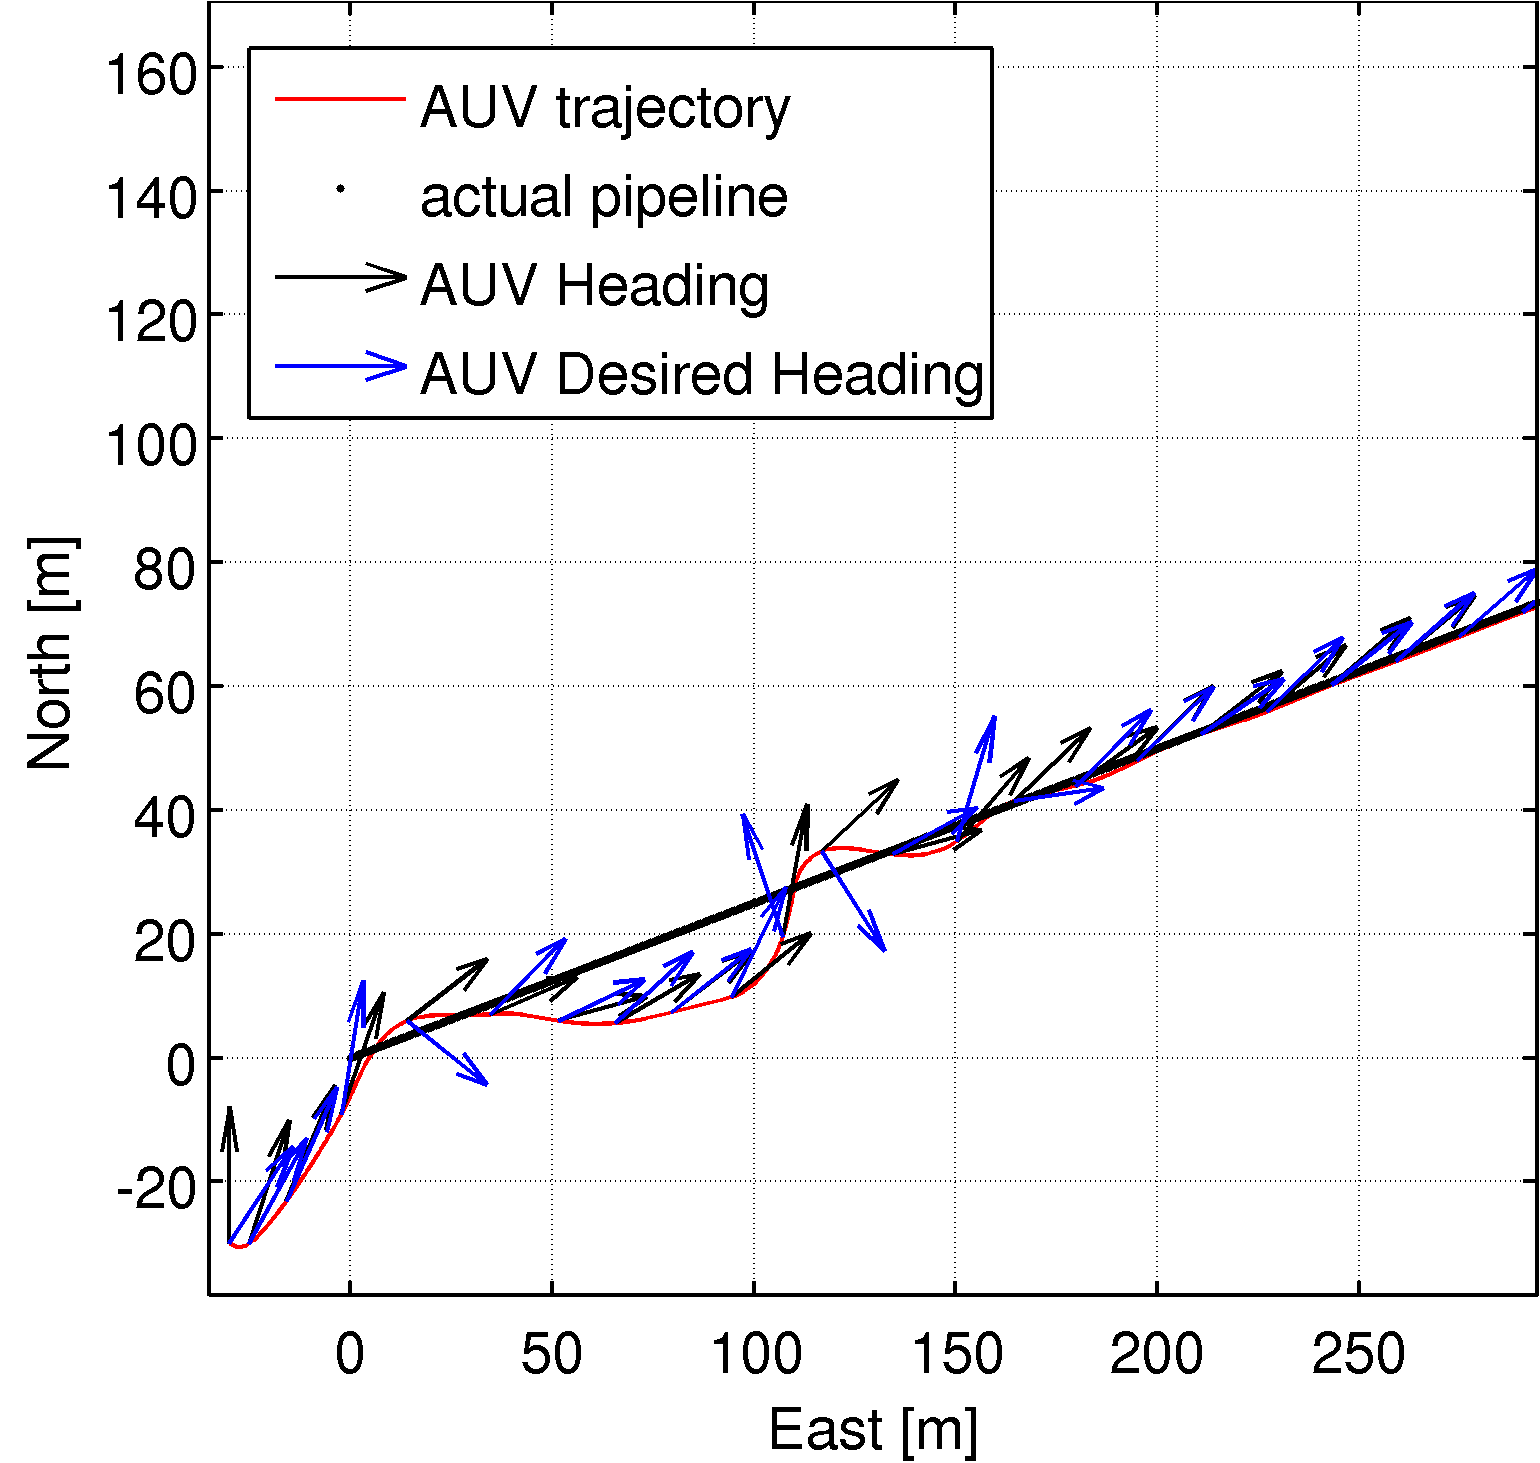
\includegraphics[width=0.5\textwidth]{pics/2nd_NE_path}} 
			\caption{Plots of the AUV Showing Trajectory, Guidance Waypoints and Heading of AUV}
			\label{fig:ch3_2nd_NE_plots}
		\end{figure}
		In Figure \ref{fig:ch3_2nd_NE_wpt} the search waypoints are shown. The reason for the extra
		``de-tour'' away from the pipeline are because of the short time delay befor considering the
		pipeline lost. As seen in the First Scenario there are oscilations in the heading reference.
		This cuases the AUV to drift off the pipeline trajectory and therefor loose visual contact
		with it. The system considers the pipeline as lost and generates a search pattern, the
		``divergent zig-zag'' spoken of in Chapter \ref{subsec:ch2_searchpattern}. The time before
		going into search mode are set to 25 seconds. This is a design parameter set by the operator.

		\begin{figure}[htbp]
			\centering
			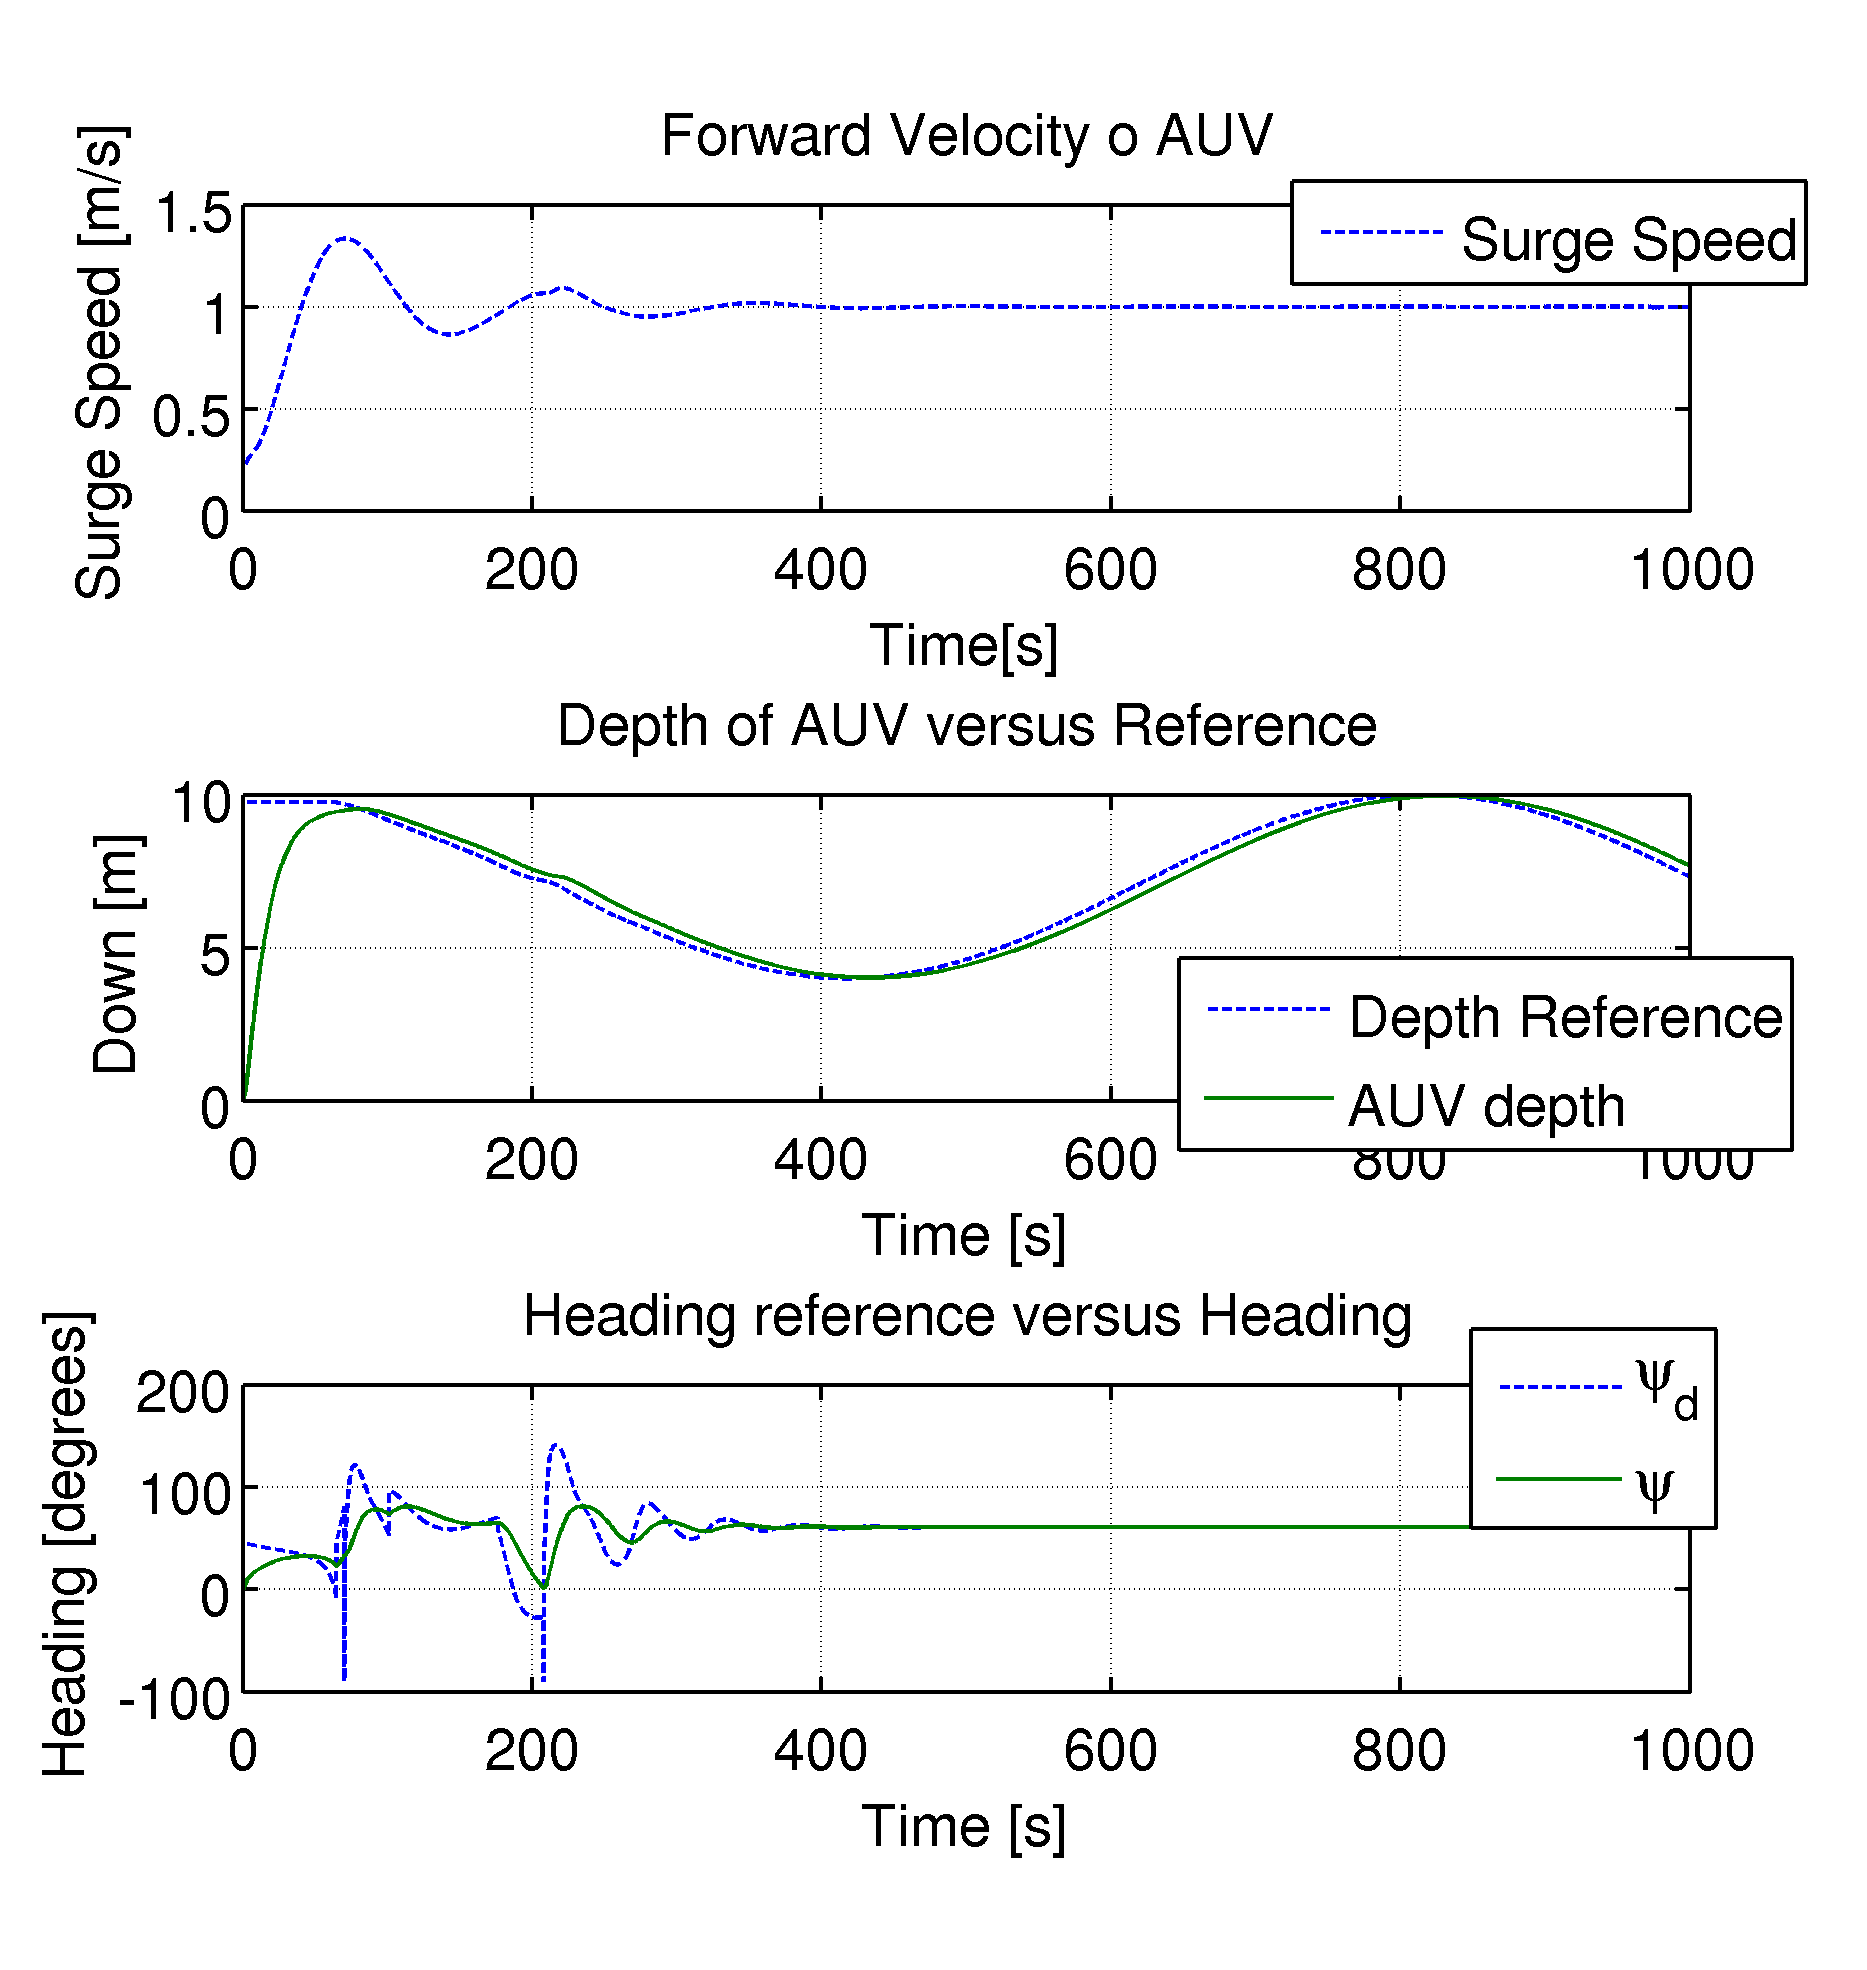
\includegraphics[width=0.70\textwidth]{pics/2nd_uDpsi}
			\caption{Surge-, Depth- and Heading- Reference with Current influence}
			\label{fig:ch3_2nd_uDpsi}
		\end{figure}
		When current are introduced the AUV heading are ``leaned'' toward the current. In Figure
		\ref{fig:ch3_2nd_NE_path} the current are coming from the north-west corder, corresponding to
		the upper right corner in the figure. This current will try to push the
		AUV off the pipeline. The guidance system answers this disturbance by adjusting the heading
		reference towards the current. This is one of the reasons why the lookahead distance are
		chosen small, because of this the AUV will no drift far away from the pipeline. Since the
		current are constant, a equilibrium will be achieved between the desired heading and the
		current. The heading converges towards around $60^{\circ}$ instead of the pipeline direction
		of $75^{\circ}$.

		The AUV are not directly on top of the pipeline anymore, but it is not desirable to be exactly
		over the pipeline all the time. To strictly control the AUV to lay exactly over the pipeline
		would use up much of the limited power supply. The objective of the AUV are not to stay
		exactly over the pipeline but to provide good pictures and sensor data for later inspections 
		by humans. 

		%\begin{figure}[htbp]
		%	\centering
		%	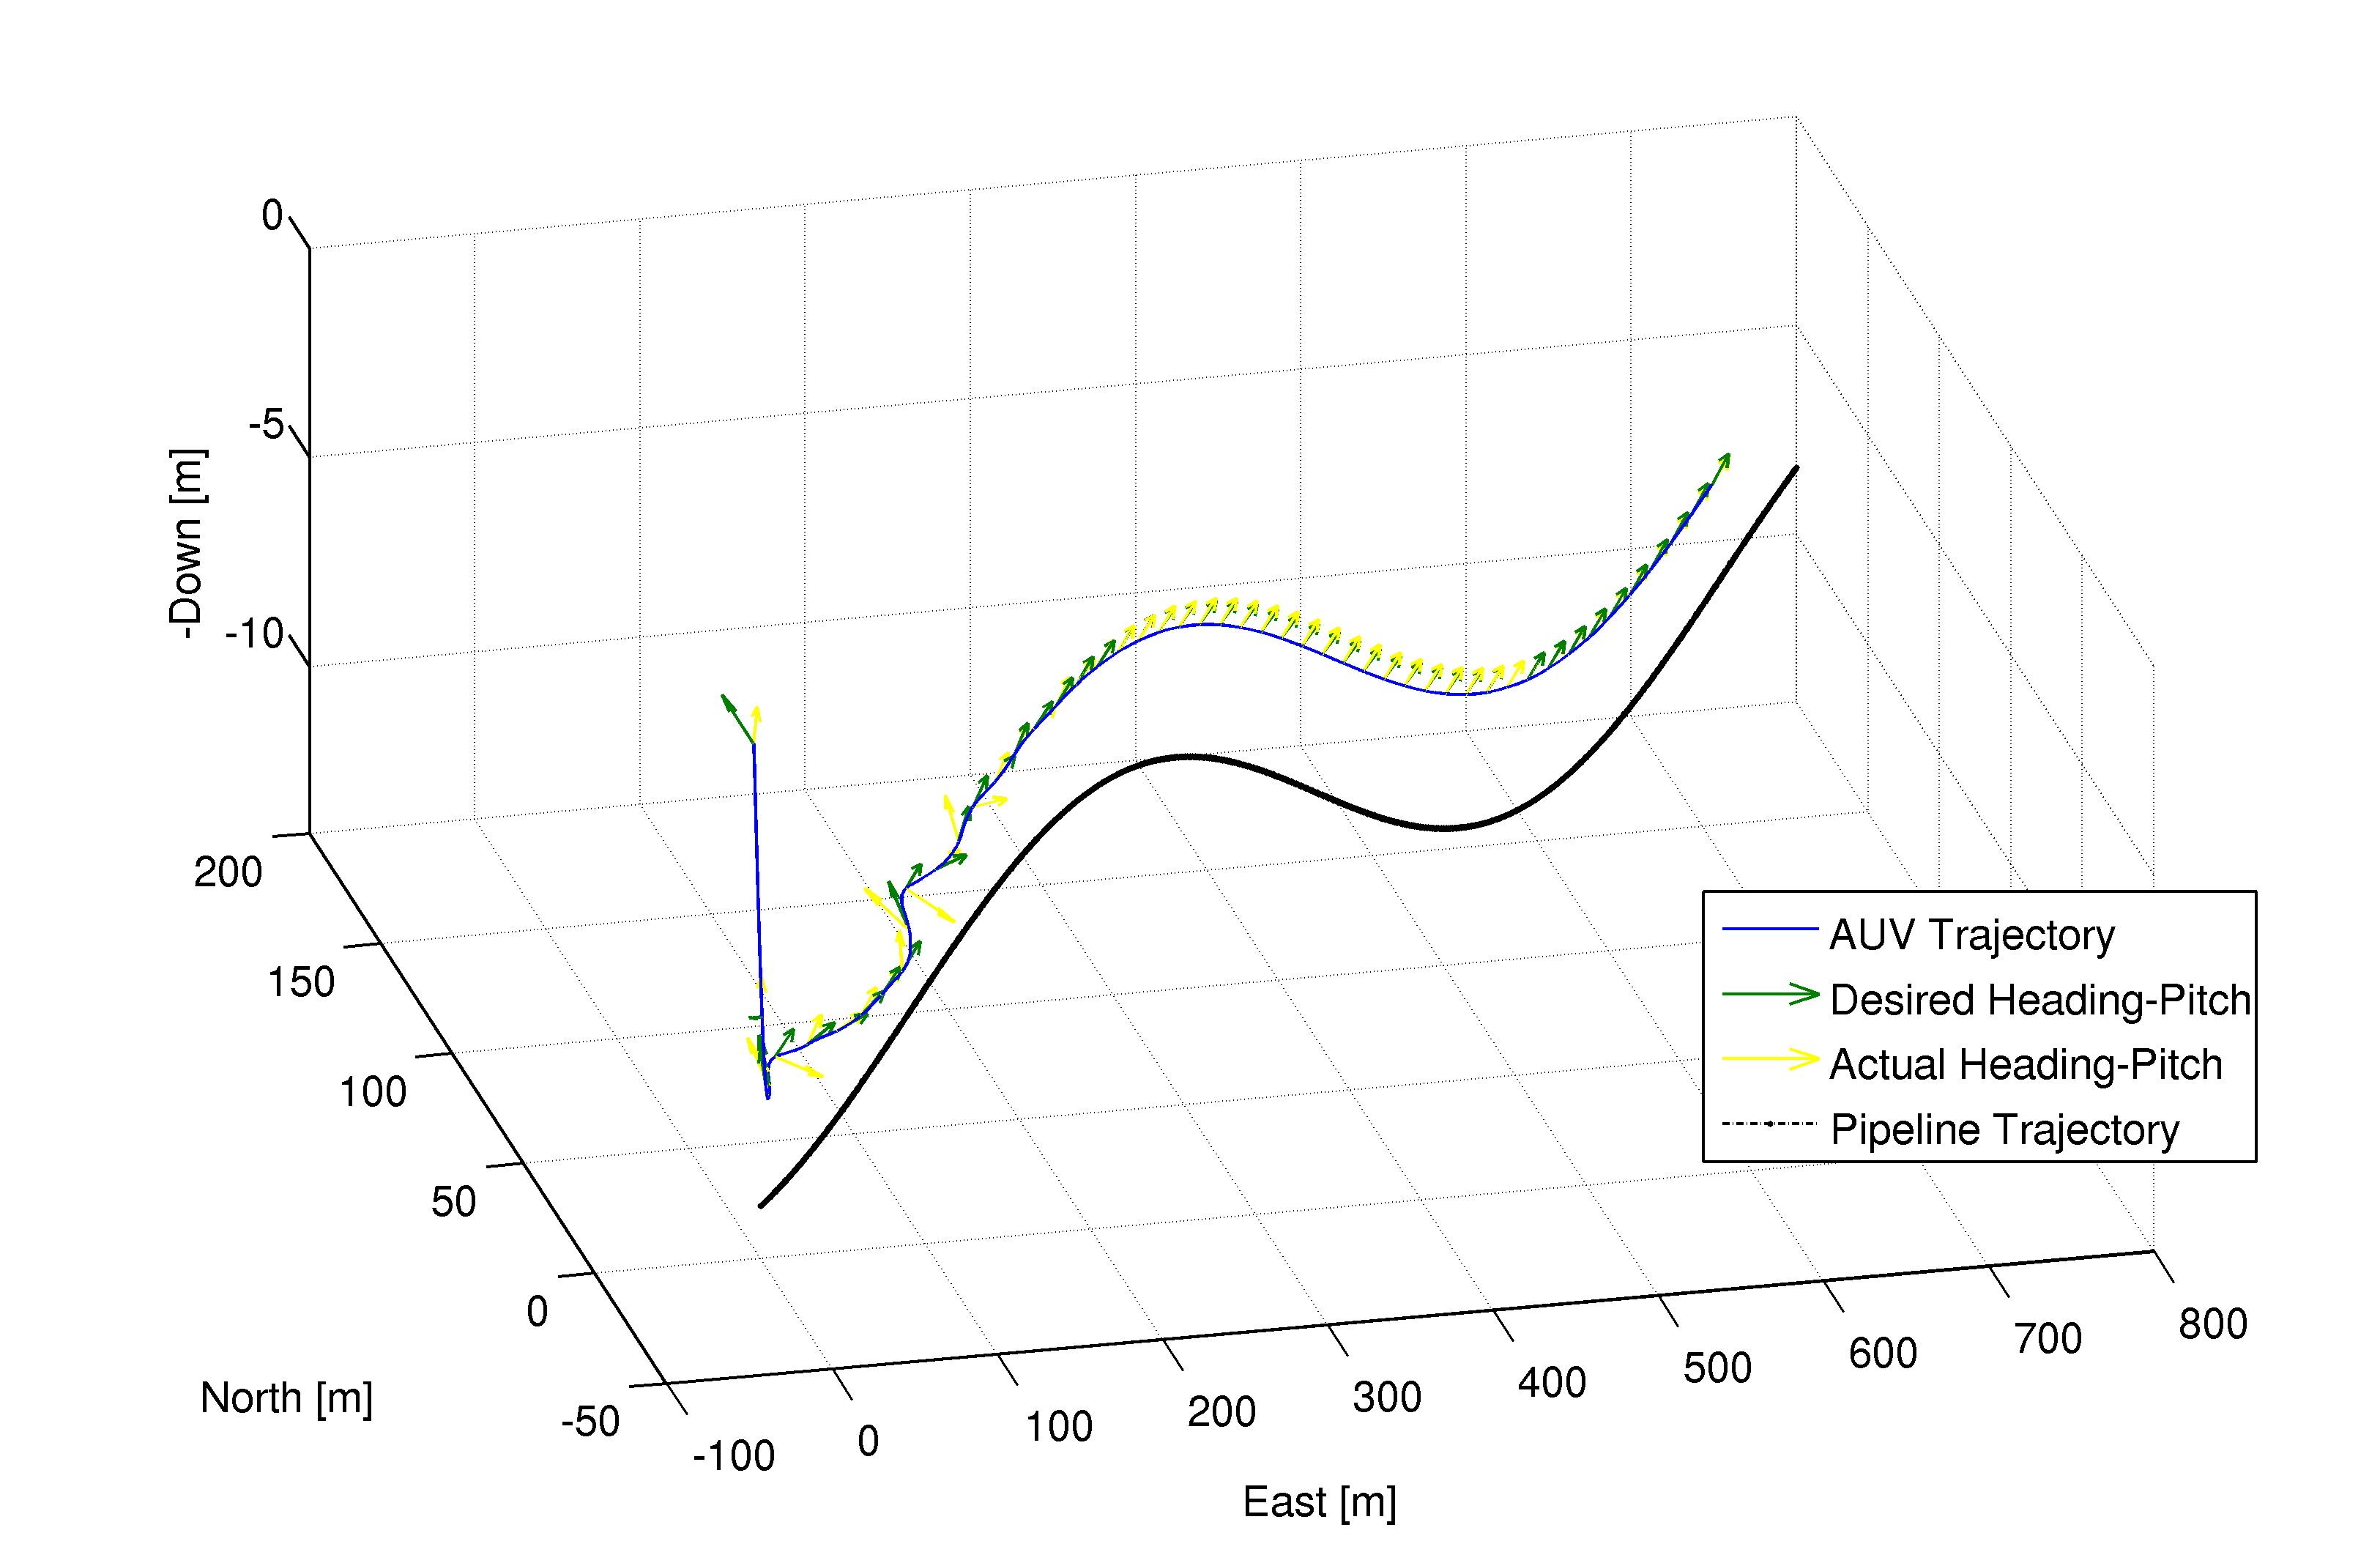
\includegraphics[width=0.95\textwidth]{pics/2nd_3d_plot}
		%	\caption{3D plot of the AUV Movement}
		%	\label{fig:ch3_2nd_3d_plot}
		%\end{figure}
		%In Figure \ref{fig:ch3_2nd_3d_plot} the 3D trajectory of the AUV are shown, togheter with the
		%actual pipeline trajectory. 
	

	\subsection{3$^{\mathrm{rd}}$ Scenario}
		The setup for this scenario, is a simulated burrial of the pipeline at apporximtley $50$
		meters North and $200$ meters East. At this point the camera looses track of the pipeline. The
		guidance system will command the AUV to continue following the predicted pipeline until some
		time limit are reached. This time limit are set to $60$ seconds. From Figure
		\ref{fig:ch3_3rd_NE_plots} it can be seen that the AUV follows the predicted pipeline for
		about $50$ meters and then engages in the predetermined search pattern.
		\begin{figure}[htbp]
			\centering
			\subfigure[NE Path with	Waypoints]{\label{fig:ch3_3rd_NE_wpt}
				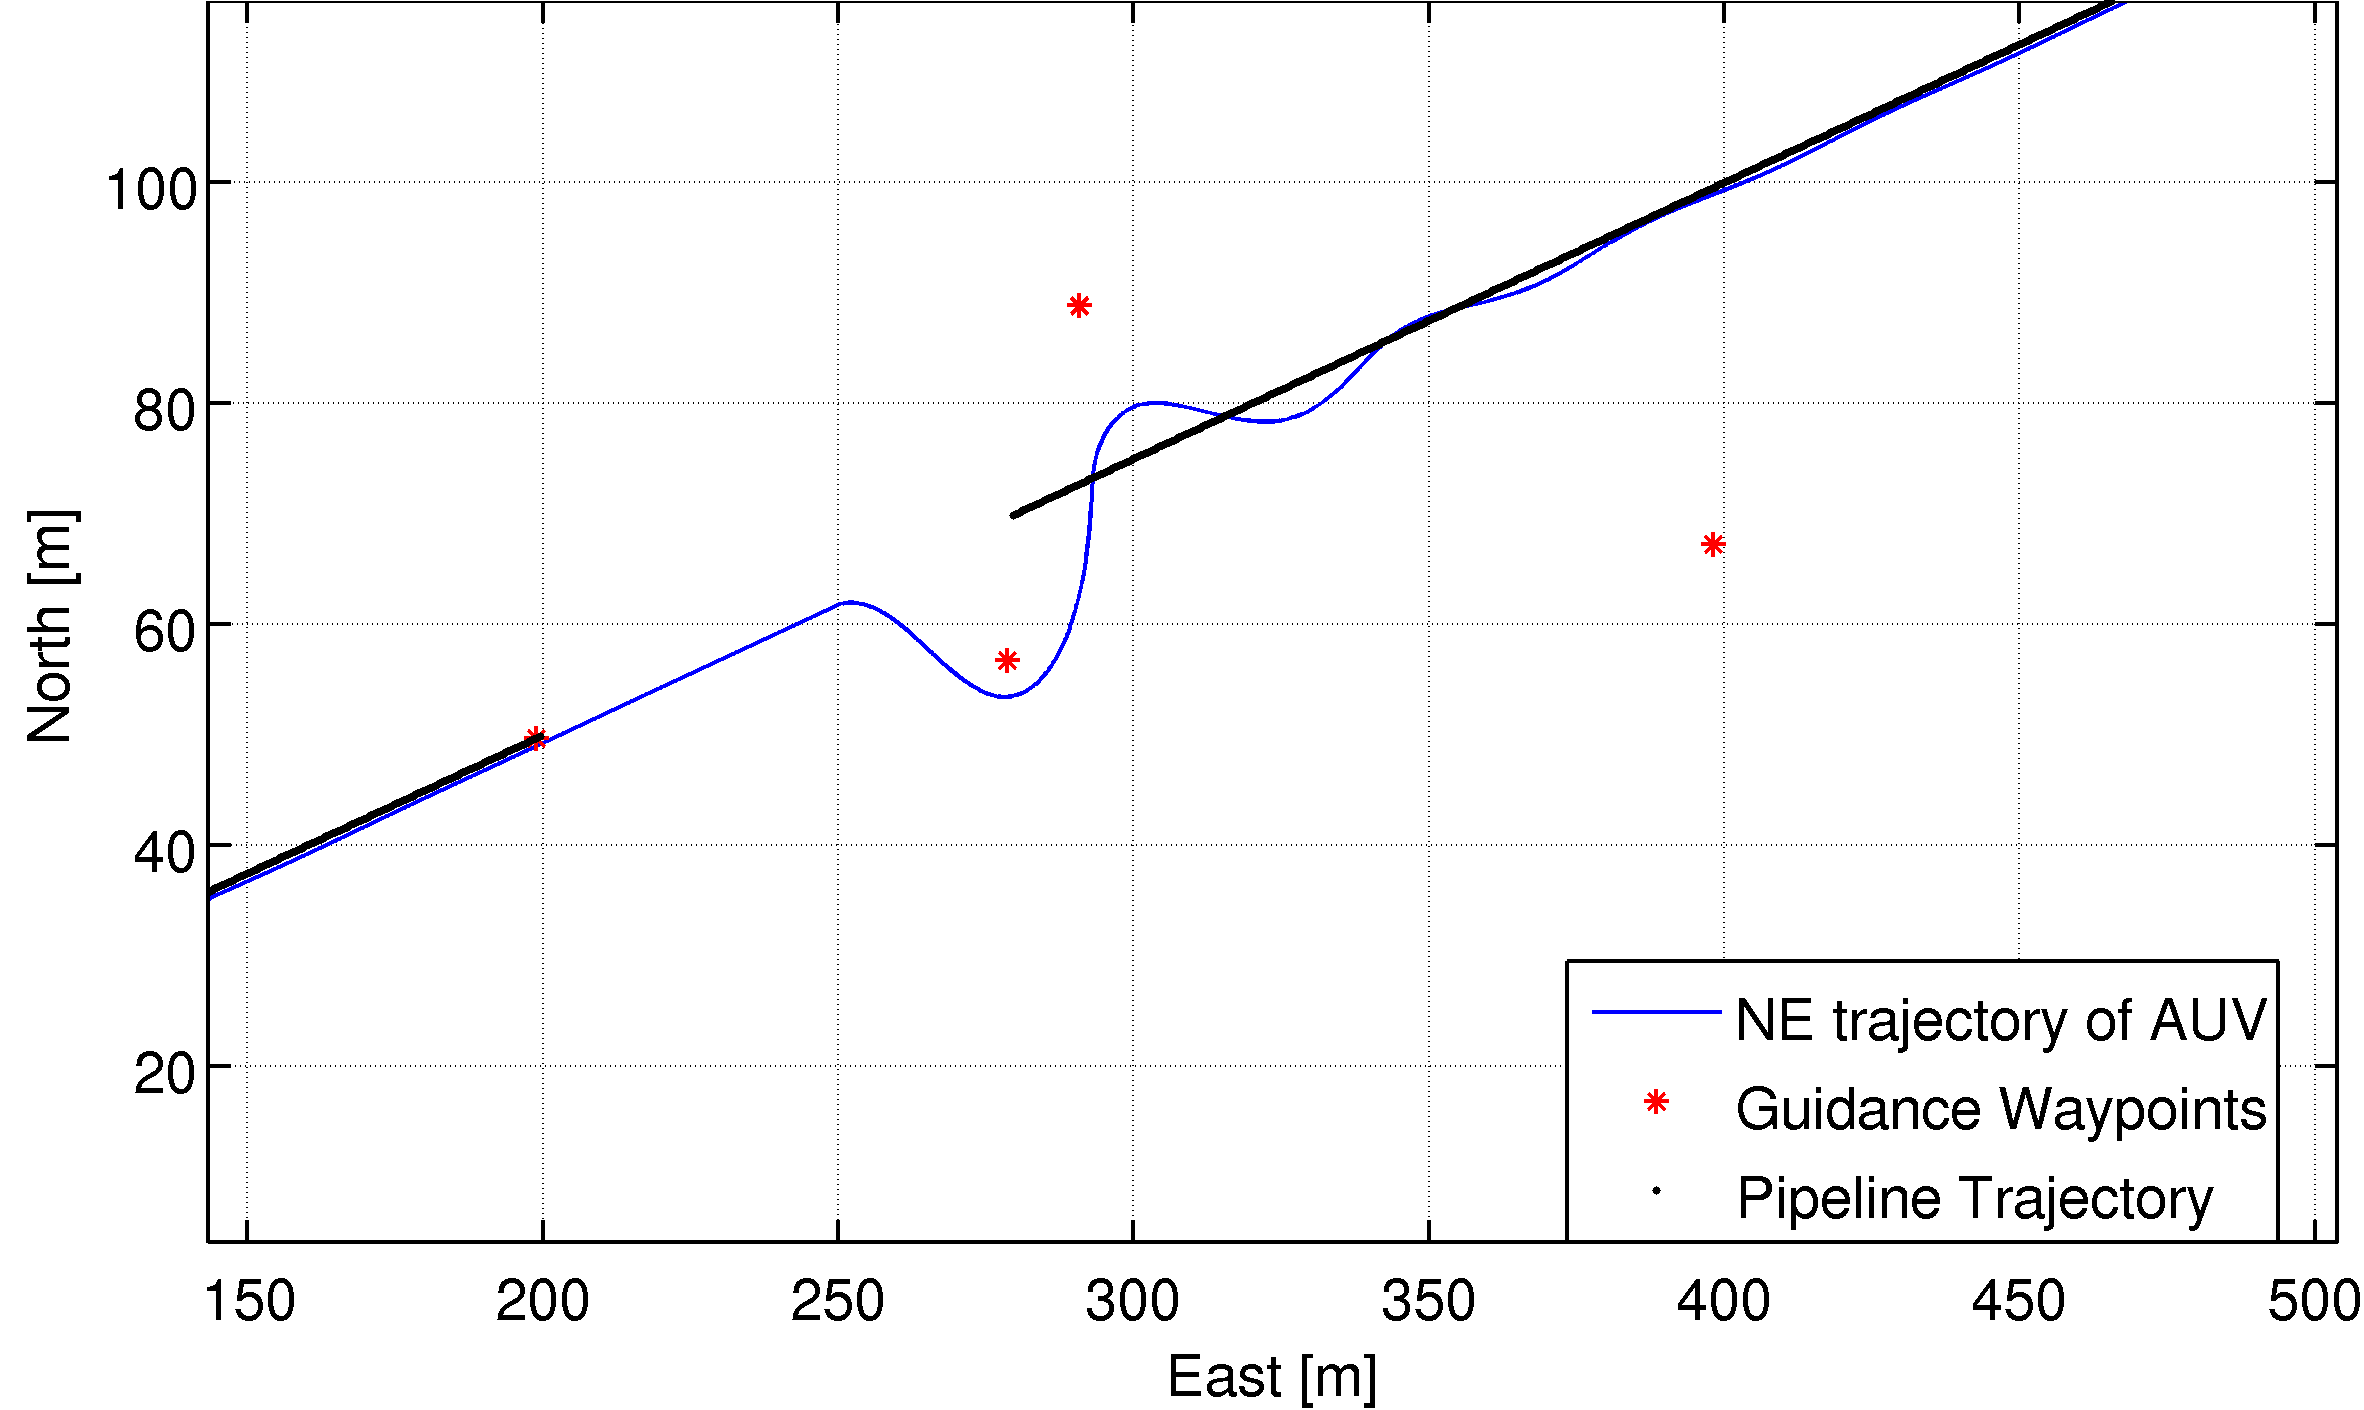
\includegraphics[width=0.7\textwidth]{pics/3rd_NE_wpt}}
			\subfigure[NE path with	Heading]{\label{fig:ch3_3rd_NE_path}
				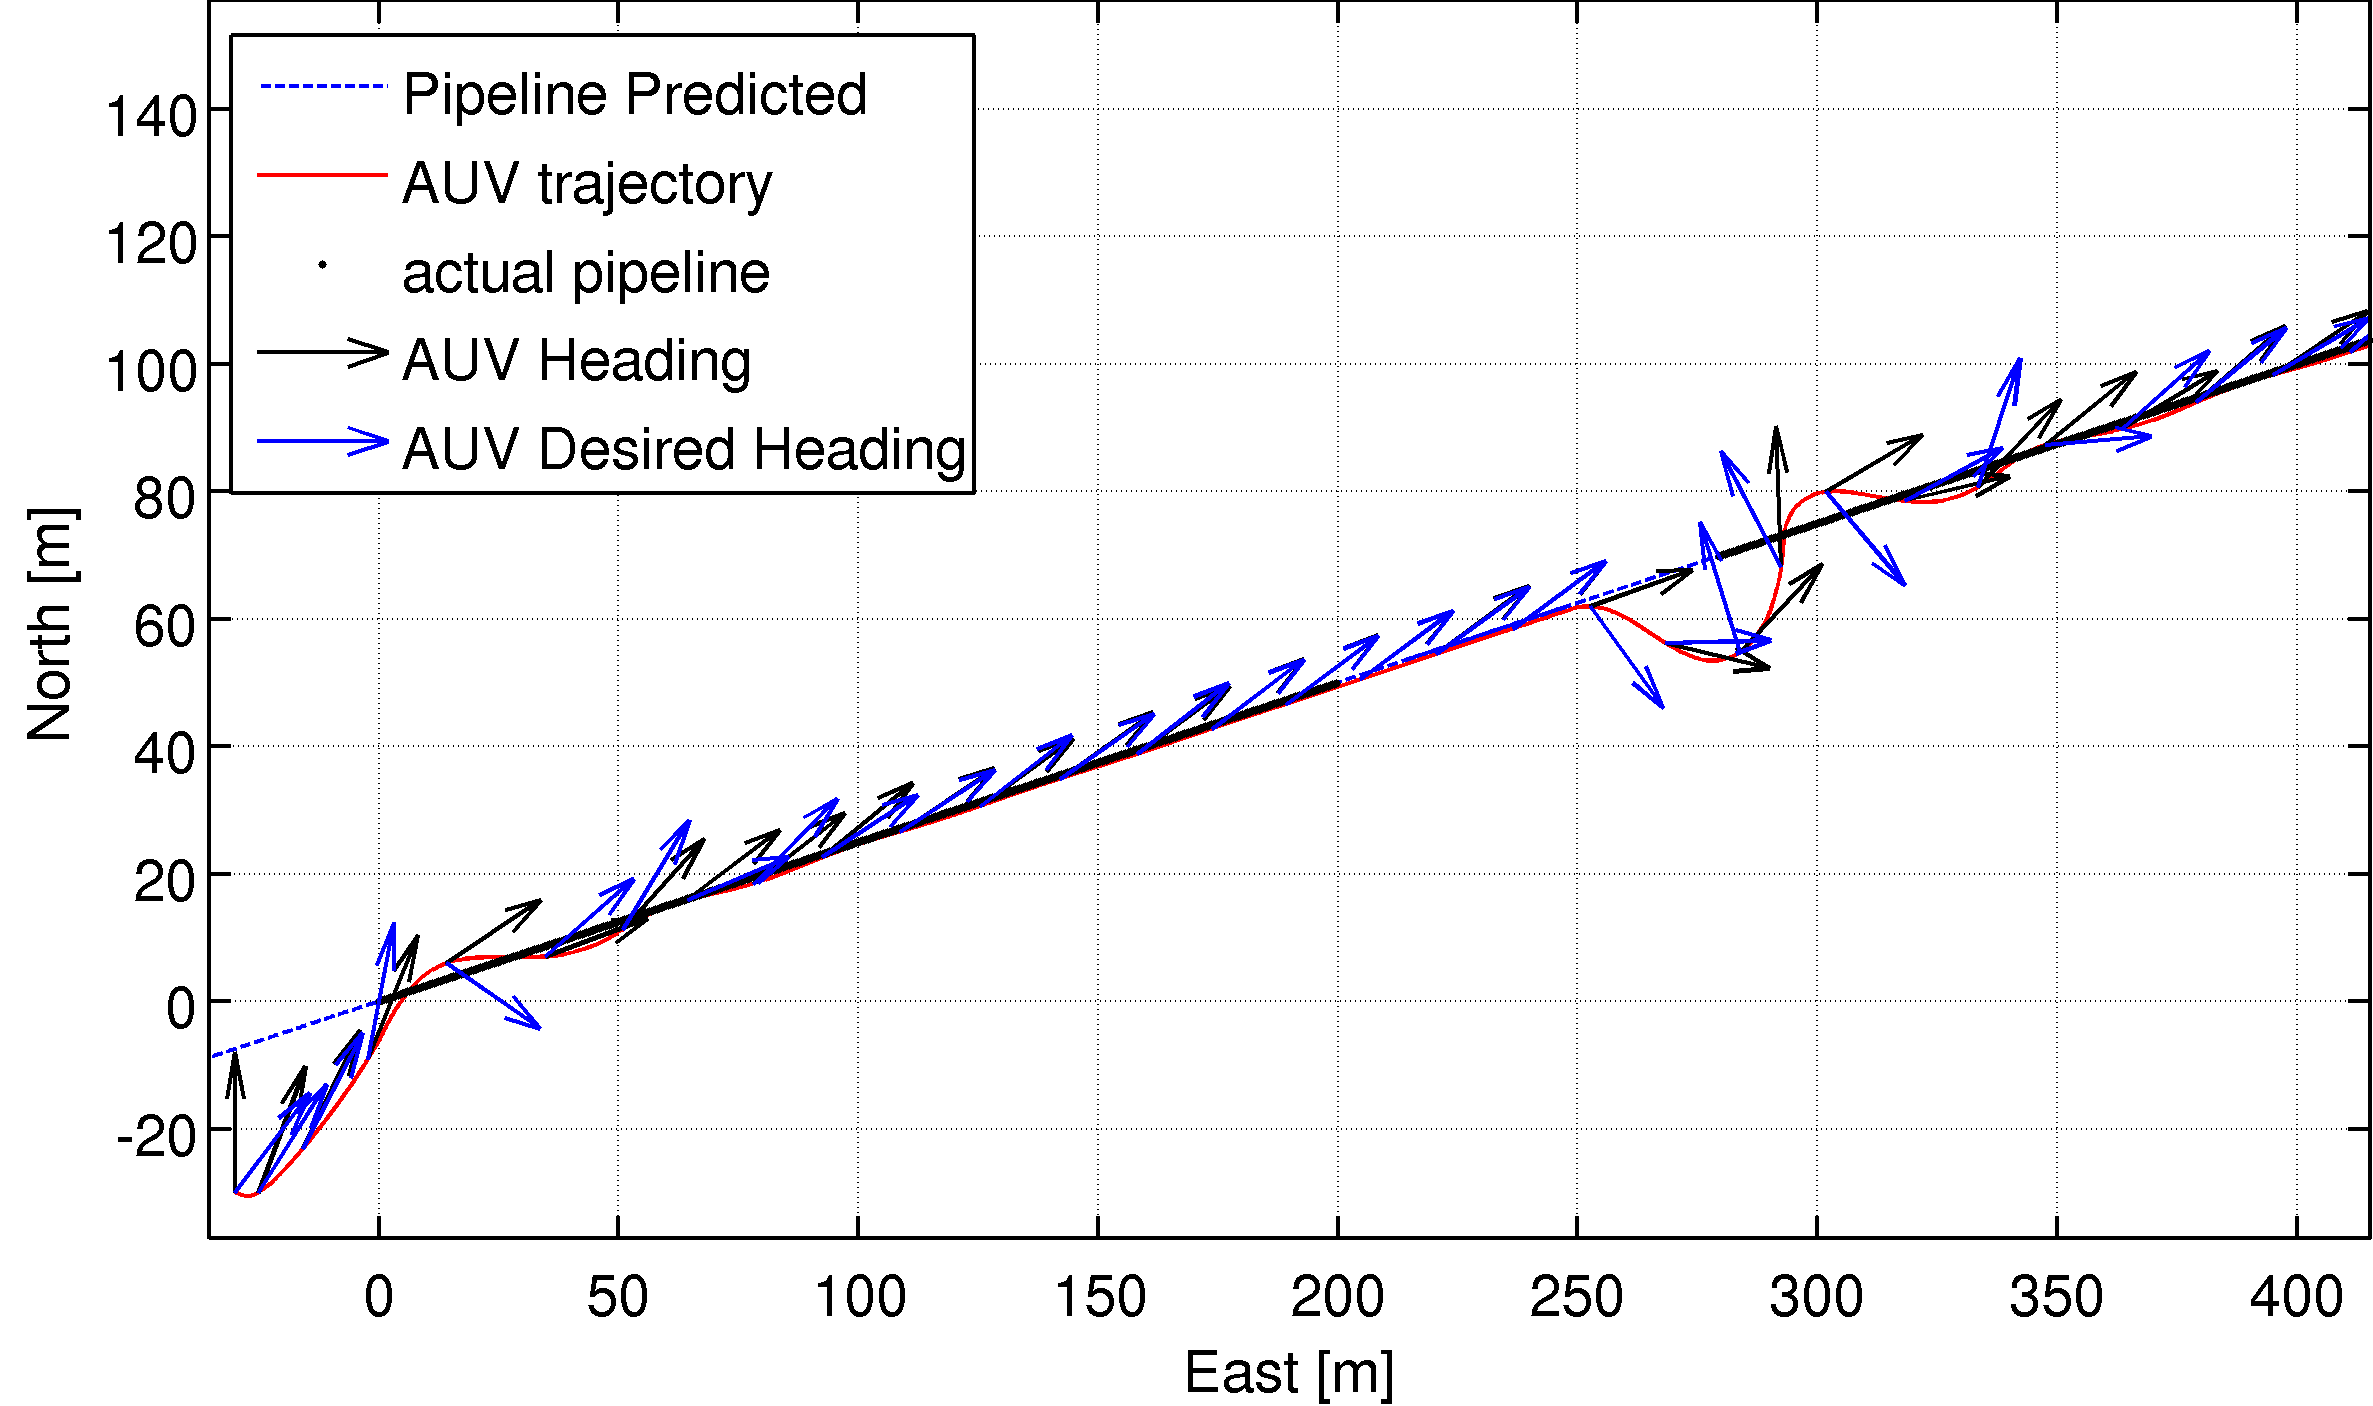
\includegraphics[width=0.7\textwidth]{pics/3rd_NE_path}} 
			\caption{Plots of the AUV Showing Trajectory, Guidance Waypoints and Heading of AUV
			for the 3$^{\mathrm{rd}}$ Scenario}
			\label{fig:ch3_3rd_NE_plots}
		\end{figure}
		
		The objective to follow the predicted pipeline is ofcourse to get back on track at the end of
		the burried strech. Sometimes pipelines are burried on purpose to seal them from environmental
		erotion, that shorten the lifetime of the pipeline. Sometimes this happens unintended. In
		either case the need for more sensors which can penetrate the sea bottom and locate the
		pipeline are needed. 
		
	
	
	\subsection{4$^{\mathrm{th}}$ Scenario}
		The fourth Scenario is to demonstrate the capabilities for the AUV to aquiere the pipeline
		when it is offset from where it was ment to be. 
		
		\begin{figure}[htbp]
			\centering
			\subfigure[NE Path with	Waypoints]{\label{fig:ch3_4th_NE_wpt}
				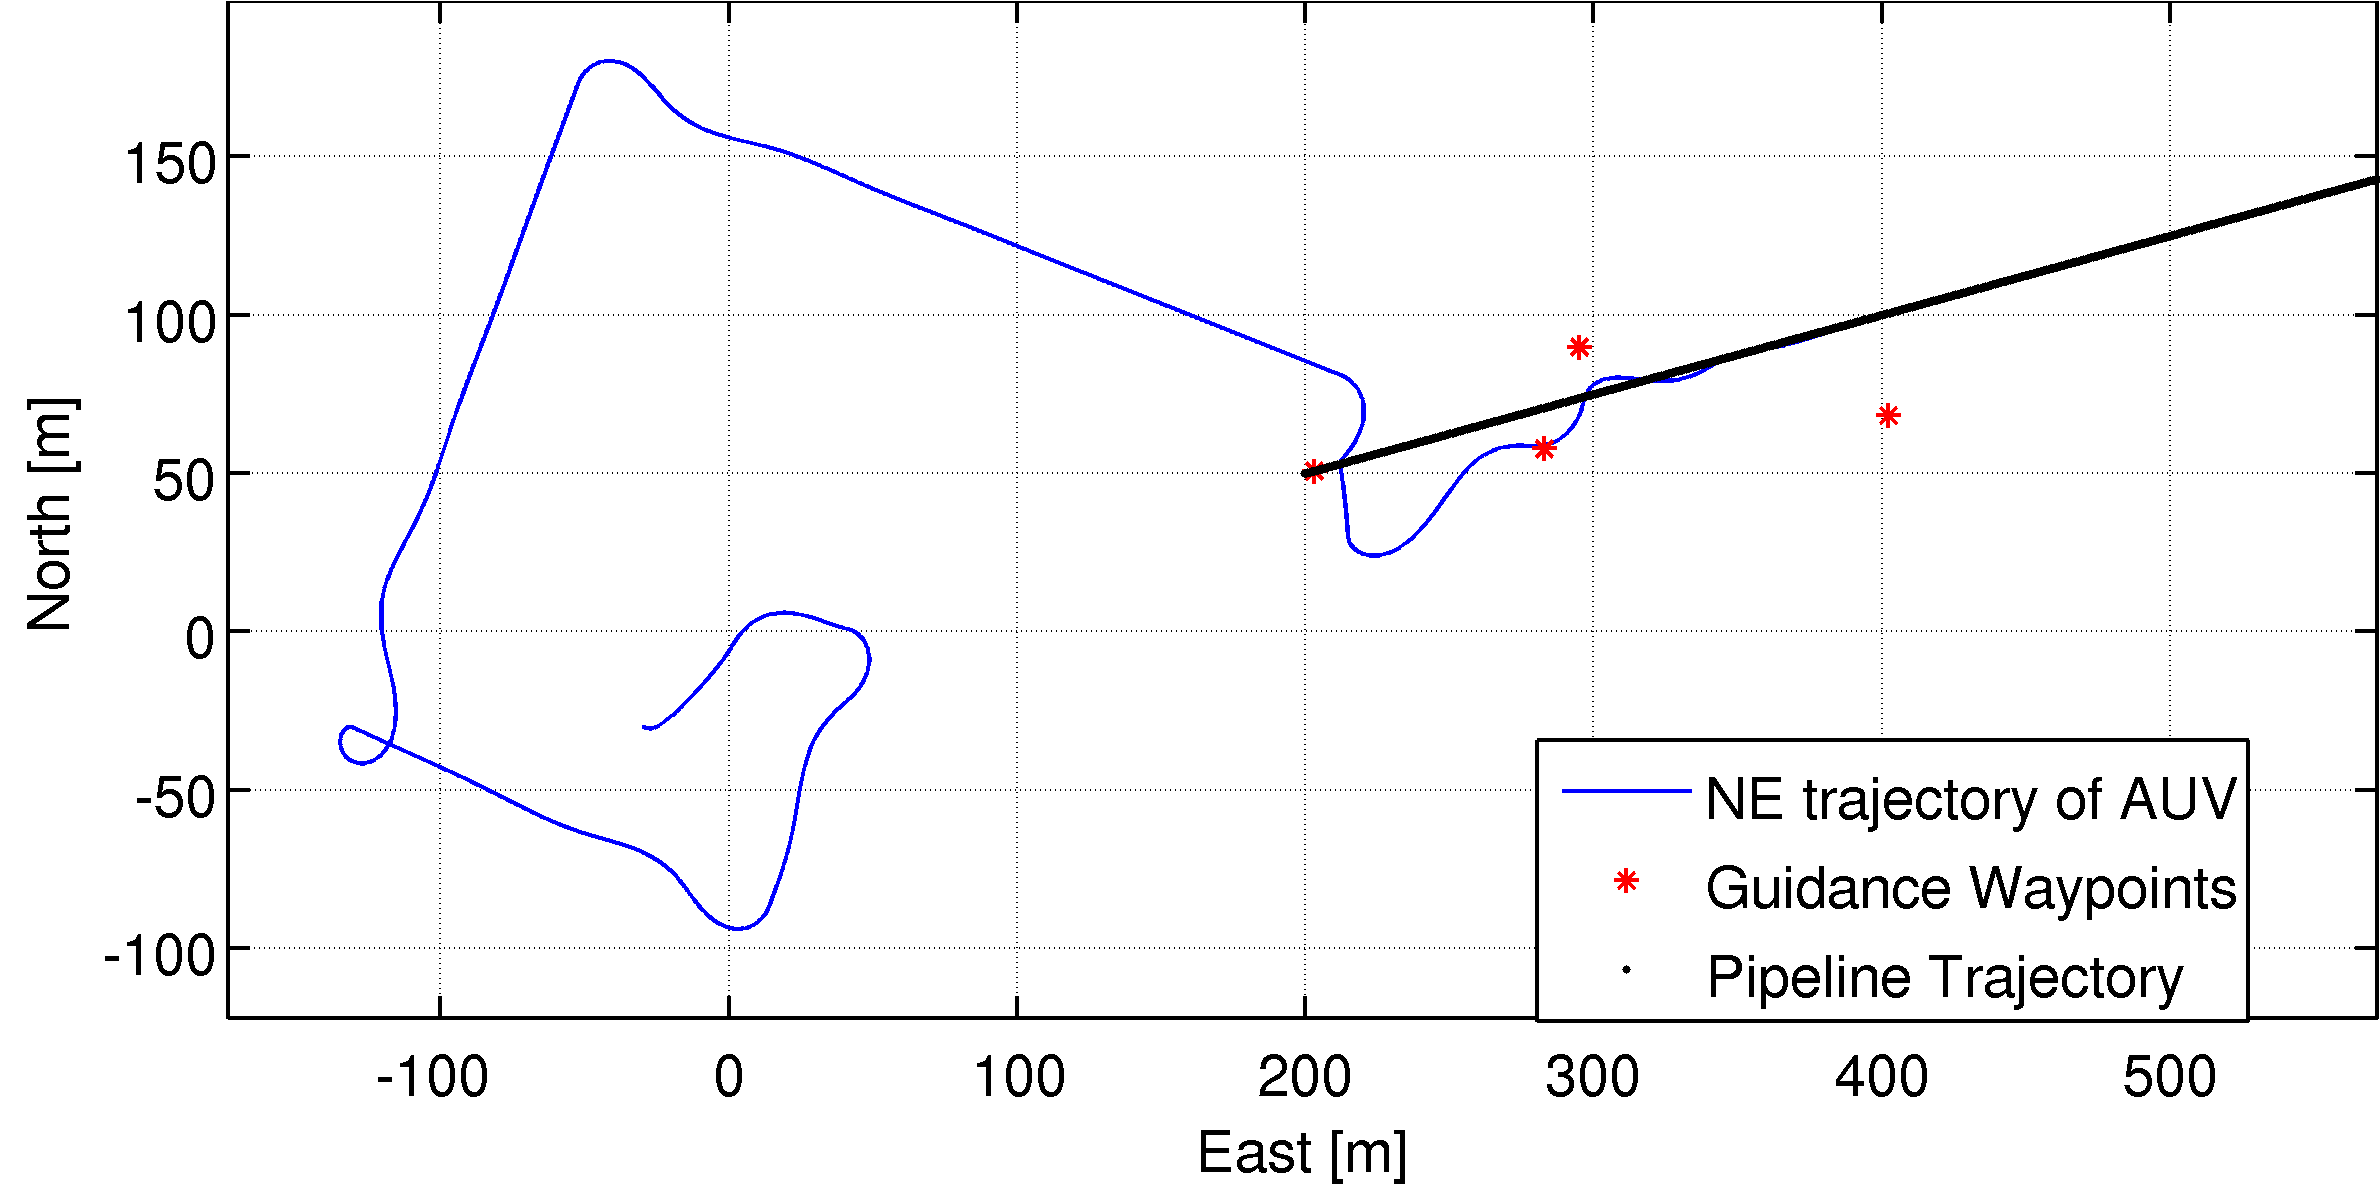
\includegraphics[width=0.8\textwidth]{pics/4th_NE_wpt}}
			\subfigure[NE path with	Heading]{\label{fig:ch3_4th_NE_path}
				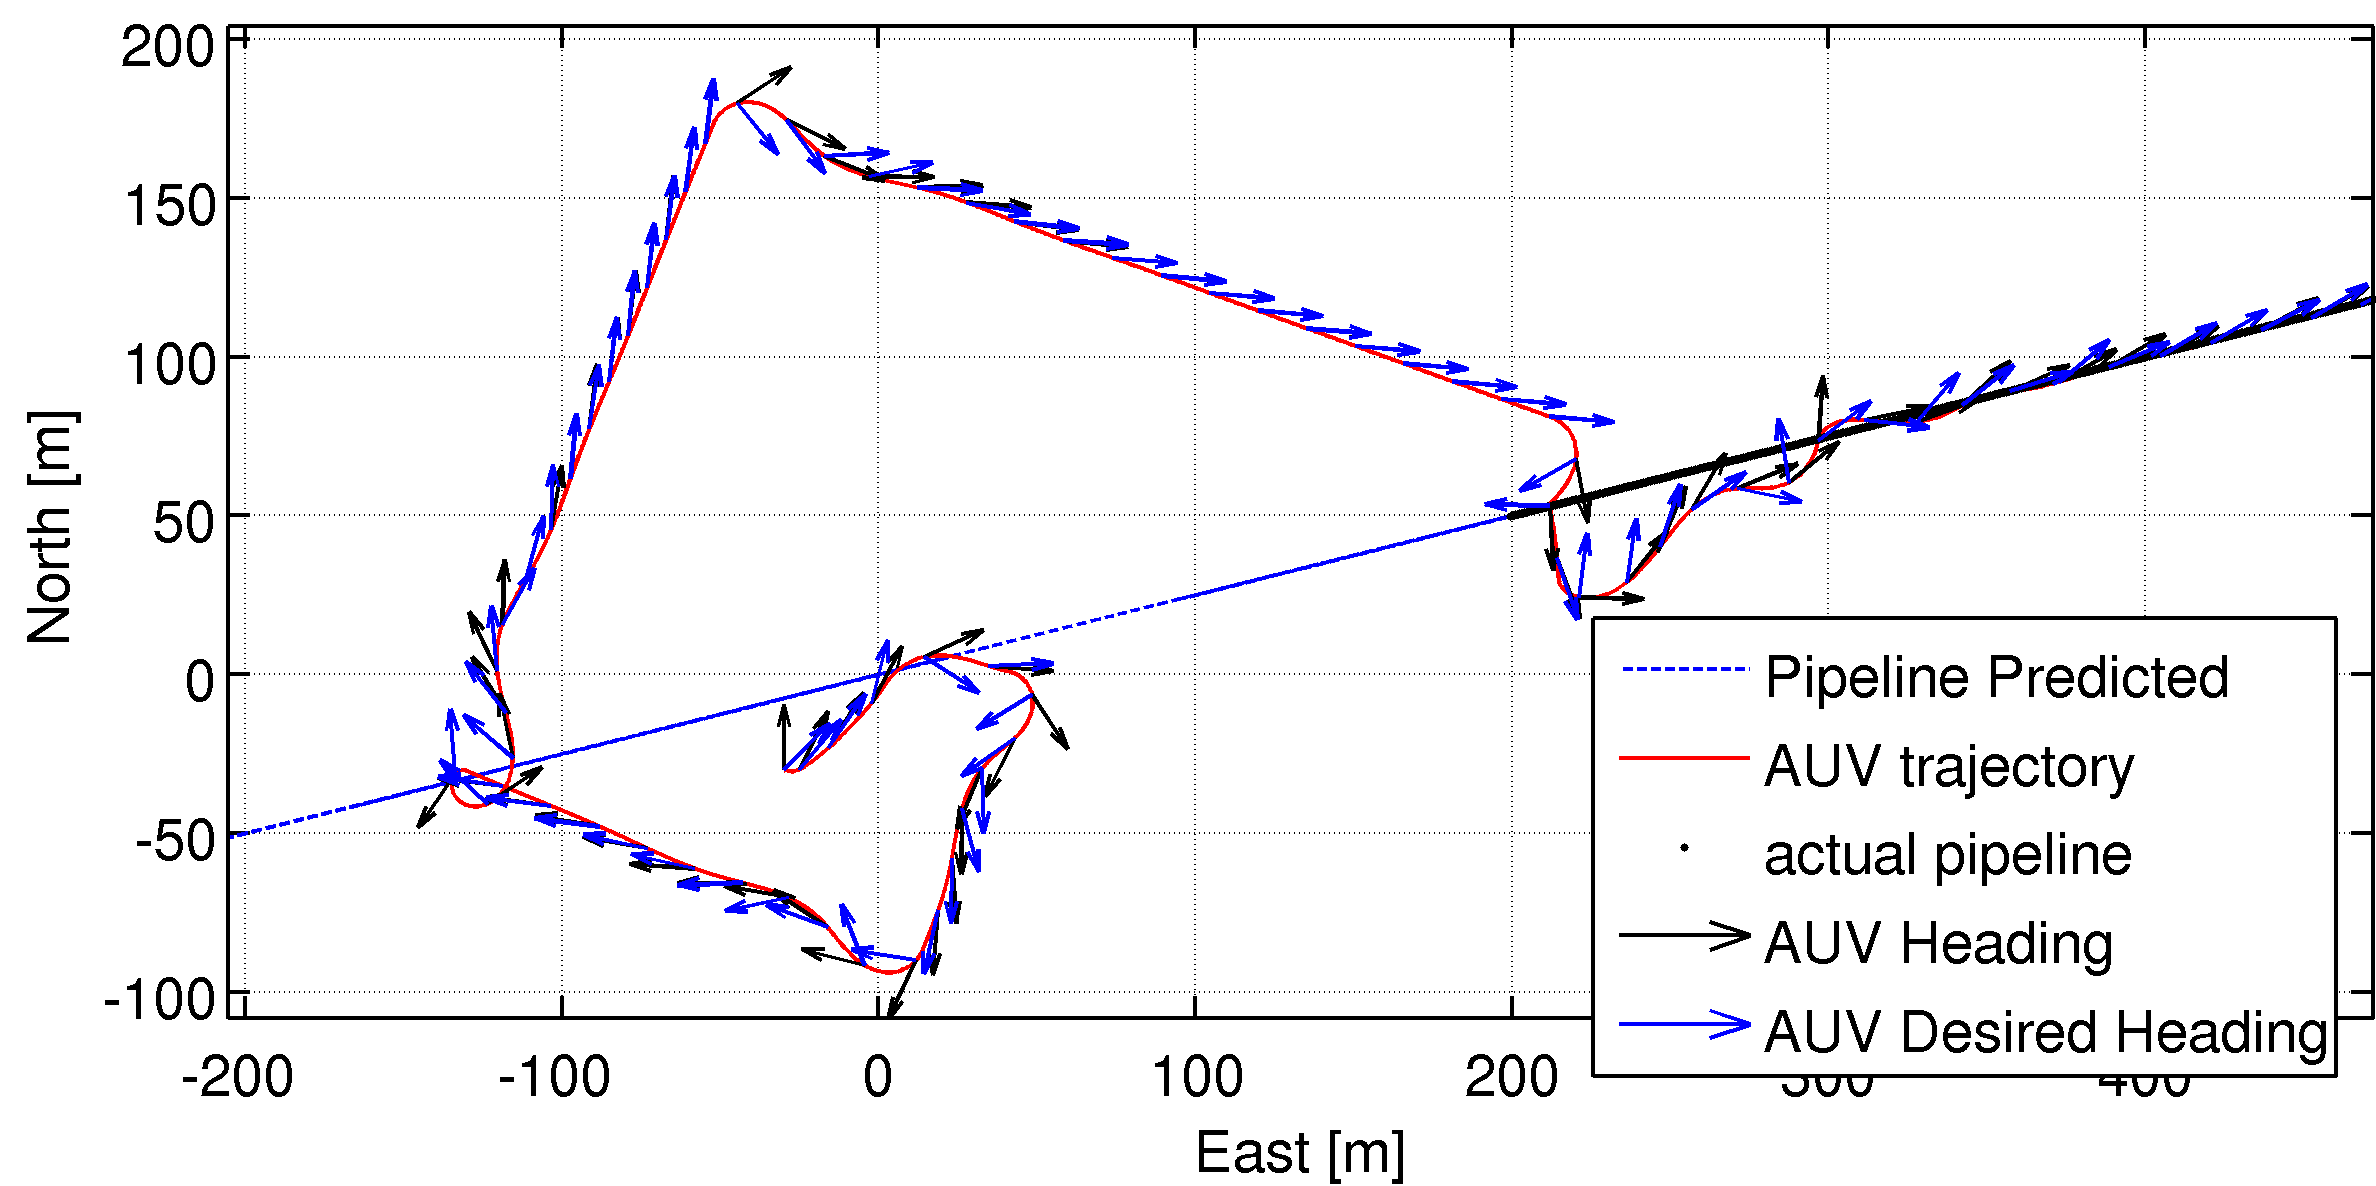
\includegraphics[width=0.8\textwidth]{pics/4th_NE_path}} 
			\caption{Plots of the AUV Showing Trajectory, Guidance Waypoints and Heading of AUV
			for the 4$^{\mathrm{th}}$ Scenario}
			\label{fig:ch3_4th_NE_plots}
		\end{figure}
		The AUV reaches the initial position where the pipeline were ment to be. It does not make
		contact with it there, then engages in a spiral search pattern. This search pattern are
		administered by waypoints and the guidance uses the straight lines between the waypoints as
		the track to follow. This causes the more polygonal look than spiral. 

		From Figure~\ref{fig:ch3_4th_NE_plots} it can be seen that the AUV sometimes takse an extra turn
		when switching between waypoint four and five. This is due to the calculation of the dersired heading
		angle. The \textit{matlab}-fucntion, \textit{atan2()} are used which outputs the angle in the
		domain $(-\pi, \pi)$. Since the output from the AUV model are defined for all values, and this
		are fed back to the controller a heading reference of 0 means that it must ``unwinde'' all
		turns it has done, because this acumulate the yaw value beyond $2\pi$.

		The large overshoot when the AUV have located the pipeline are due to the current. This
		pushes the AUV away from the trajectory. The current increases the velocity in a direction and
		causes the turning in that direction to be more difficult than turning the other way. 



		


